
\FloatBarrier

\section{Система Лоренца} %  % {{{1 _LOR_
\label{atu:sect:lor}

\LinkRef{
  lor: ASAU-22, 23, 24, 25, 26.
  % ~/doc/tex/asau/asau22/atu/atu.tex
  % ~/doc/tex/asau/asau23/atu/atu.tex
  % ~/doc/tex/asau/asau24/atu/atu.tex
  APIR-2012. CSIT-2015. ISDMCI-2014, ISDMCI-2015.
  ITMM-2012, ITMM-2014, ITMM-2015, DSMP-2016
}

\subsection{Определение системы и анализ её динамики} %  % {{{2 _LOR_task

В качестве первой идентифицируемой хаотической системы рассмотрим классическую
систему Лоренца, динамика которой описывается системой
уравнений~\cite{moon_chaotic_vibr,anisch_nonlin_eff,chulichkcov_mm_ml_dyn,berje_order_in_chaos}:
%
\begin{equation}
\begin{cases}
  \dot{x} = \sigma (y-x ) , \\
  \dot{y} = x (r-z) - y , \\
  \dot{z} = x y - b z .
\end{cases}
\label{atu:eq:lor}
\end{equation}

Наиболее ценным с точки зрения идентификации является параметр
$r$, определяющий как энергетическое состояние системы,
так и вид динамики системы.
Это подтверждают
рассмотренные в дальнейшем физические обоснования.
Для определённости зададим остальные параметры следующим классическим образом:
$b = 2.6666667$, $\sigma = 10$, если не будет явно указано обратное.


При малых значениях параметра $r$ система демонстрирует
затухающие колебания (рис.~\ref{atu:f:lor_attractor_fading}).

\begin{figure}[ht!]
\begin{center}
  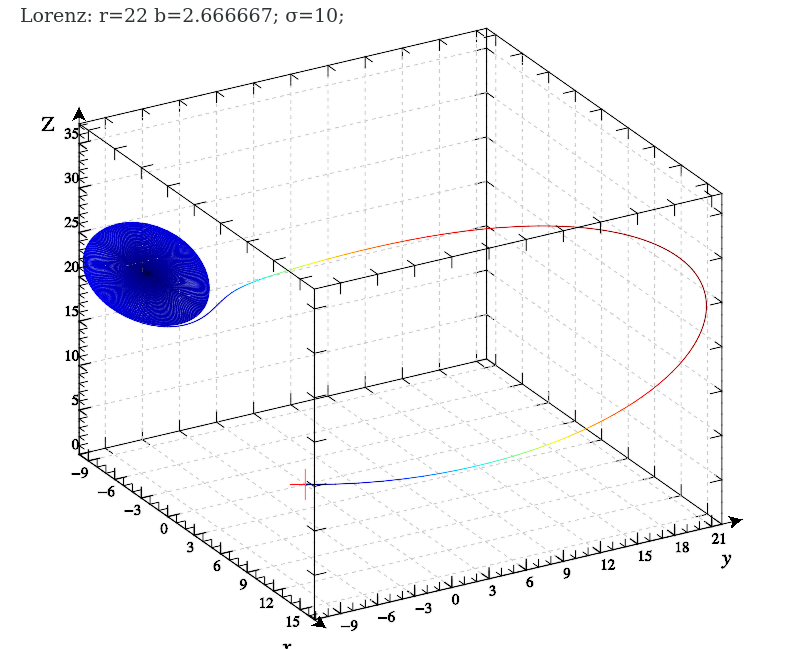
\includegraphics[width=0.49\textwidth]{p/cha/lor/lor0-p_xyz_r=022.png}
  \hfill
  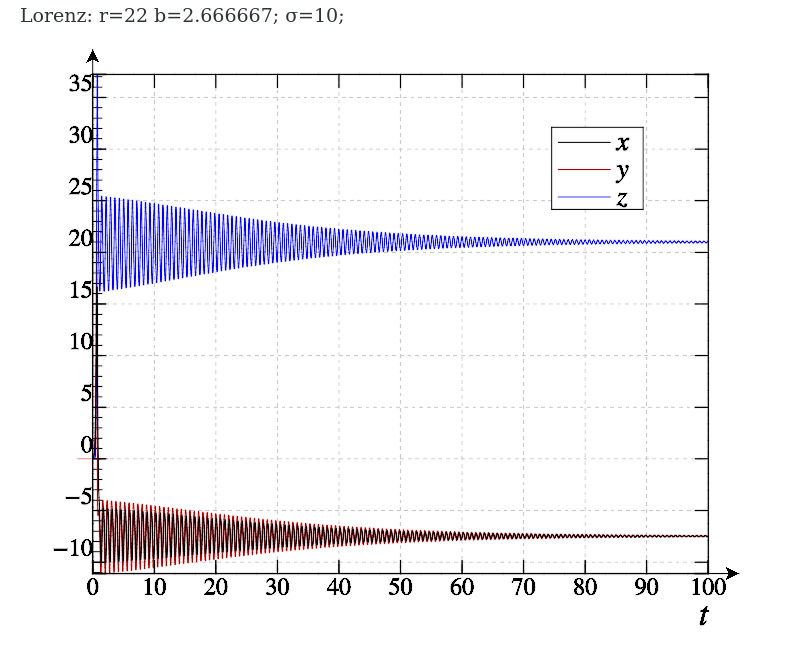
\includegraphics[width=0.49\textwidth]{p/cha/lor/lor0-p_t_r=022.png}
\end{center}
  \caption{Аттрактор и поведение переменных состояния системы Лоренца (\ref{atu:eq:lor}) в режиме затухающих колебаний ($r=22$)}
\label{atu:f:lor_attractor_fading}
\end{figure}

Далее,  в широком диапазоне значения параметра $r$
система проявляет хаотическую динамику. Помимо
этого, спектр данной системы в хаотическом режиме довольно широк
(рис.~\ref{atu:f:lor_attractor_phase_chaos28})
и не имеет доминирующих частот, что не характерно для многих систем
динамического хаоса.

\begin{figure}[ht!]
\begin{center}
  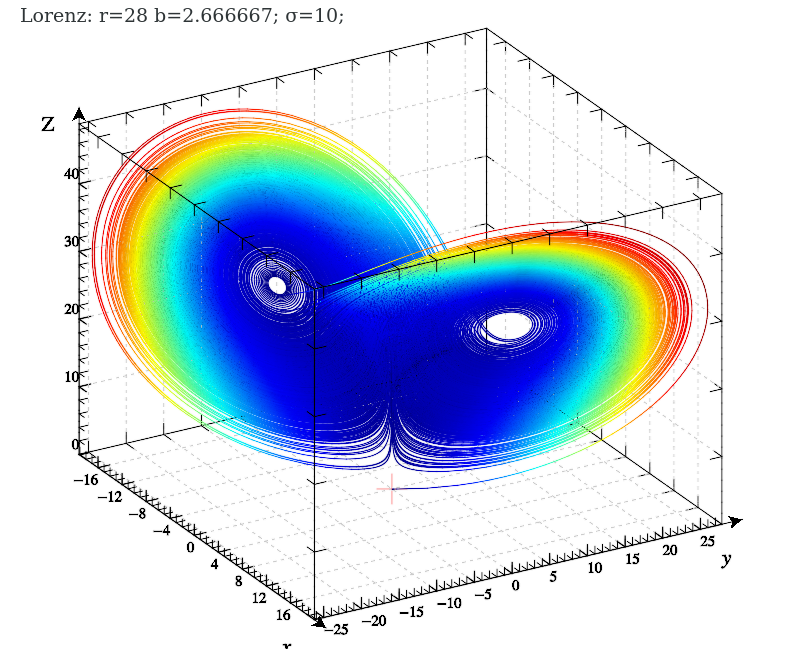
\includegraphics[width=0.49\textwidth]{p/cha/lor/lor0-p_xyz_r=028.png}
  \hfill
  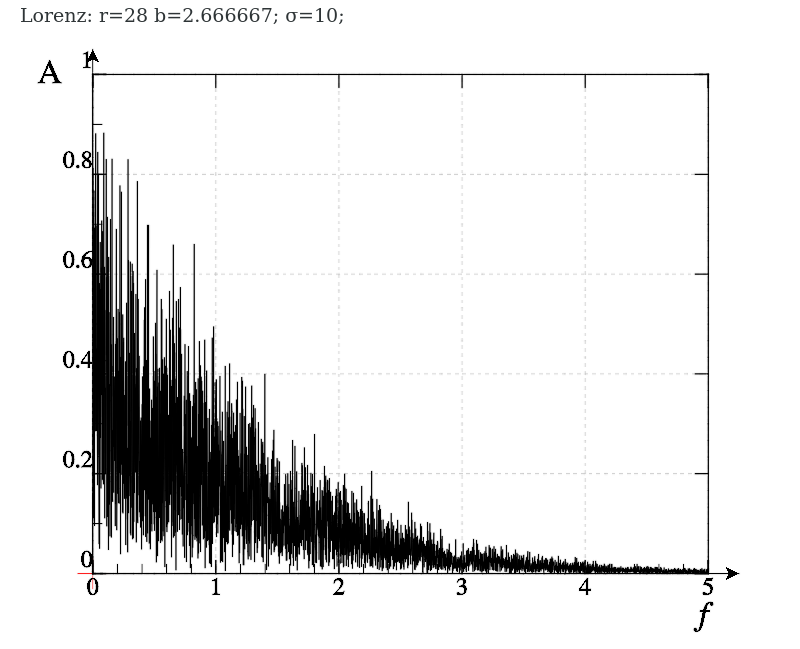
\includegraphics[width=0.49\textwidth]{p/cha/lor/lor0_fft-p_f_r=028.png}
\end{center}
  \caption{Аттрактор и спектр системы Лоренца (\ref{atu:eq:lor}) в хаотическом режиме ($r=28$)}
\label{atu:f:lor_attractor_phase_chaos28}
\end{figure}

При дальнейшем росте параметра $r$ динамика системы становится
сложно-периодической, с явно выраженным линейчатым спектром
(рис.~\ref{atu:f:lor_attractor_phase_200})

\begin{figure}[ht!]
\begin{center}
  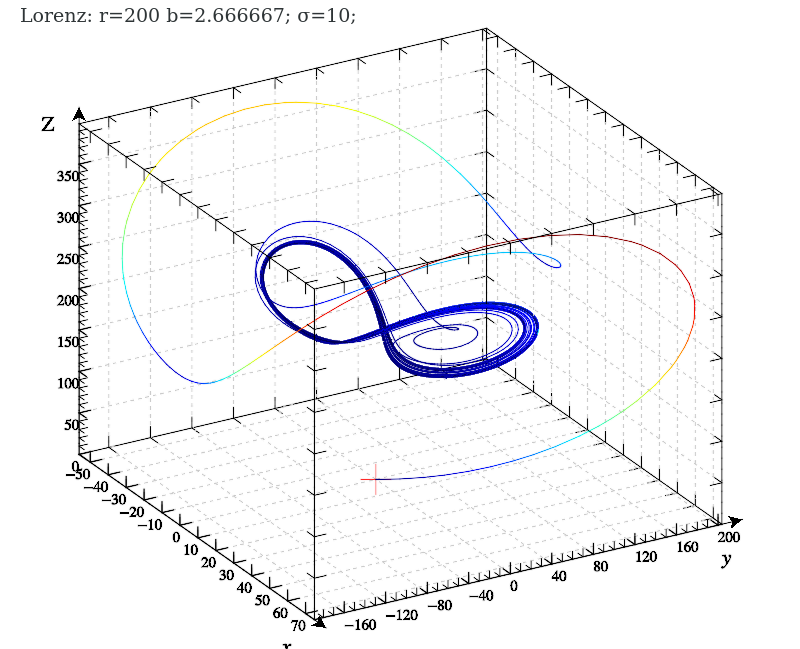
\includegraphics[width=0.49\textwidth]{p/cha/lor/lor0-p_xyz_r=200.png}
  \hfill
  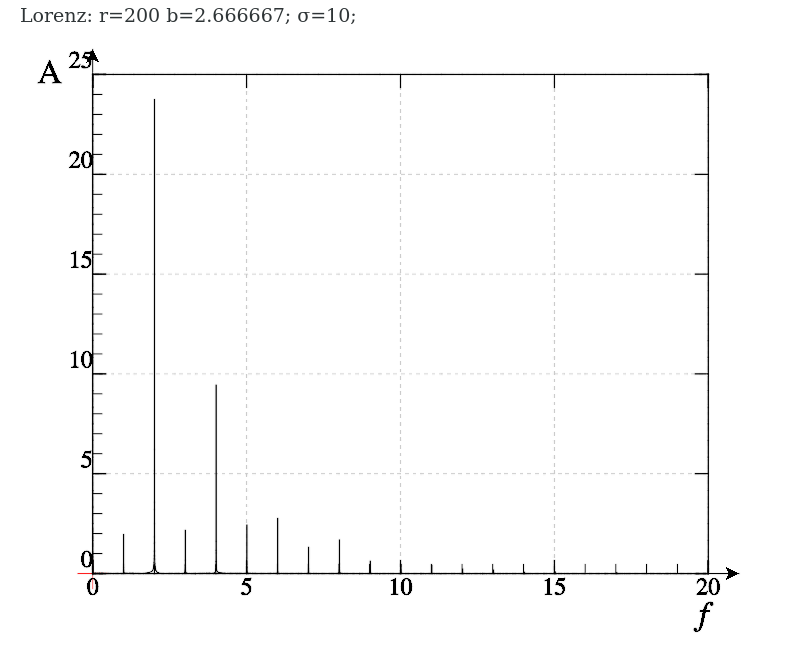
\includegraphics[width=0.49\textwidth]{p/cha/lor/lor0_fft-p_f_r=200.png}
\end{center}
  \caption{Аттрактор и спектр системы Лоренца (\ref{atu:eq:lor}) в сложно-периодическом режиме ($r=200$)}
\label{atu:f:lor_attractor_phase_200}
\end{figure}



Динамическая система Лоренца является одной из наиболее изученных
хаотических систем~\cite{neimark_stoch_chaos_vibro}. % TODO: more
При этом, существует множество физических систем, для
описания которых применима модель Лоренца. Это дает определённые основания
предполагать, что синтез критерия идентификации, основанного на физических
принципах, для данной системы будет успешным.


Для синтеза критерия идентификации параметра $r$ системы (\ref{atu:eq:lor}), рассмотрим
набор физических систем, для моделирования которых применяется система
Лоренца.

Исторически первой такой системой, рассмотренной самим Лоренцом, является
задача о тепловой конвекции жидкости в плоском слое. Исходная система
уравнений гидродинамики имеет вид:
%
%
\begin{equation}
\begin{cases}
  \pd{\vec{v}}{t} + ( \vec{v} \nabla ) \vec{v} = - \frac{\nabla p}{\rho} + \nu \Delta \vec{v} + \vec{g}, \\
  \pd{\rho}{t} + \nabla ( \rho \vec{v} ) = 0 , \\
  \pd{T}{t} +\nabla ( T \vec{v} ) = \chi \Delta T , \\
  \rho = \rho_0 \left( 1 - \gamma (T - T_0) \right) .
\end{cases}
\label{atu:eq:lor_gidro}
\end{equation}
%
где
$\vec{v} $   --- поле скоростей,
$T$ --- поле температуры,
$T_0$ и $T_0+\Delta T$   --- температуры на верхней и нижней границе соответственно,
$\rho$ и $p$ --- поля плотности и давления,
$g$ --- ускорение свободного падения,
$\nu$, $\chi$, $\gamma$  --- коэффициенты кинематической вязкости, температуропроводности и
теплового расширения соответственно.

При приближении системы (\ref{atu:eq:lor_gidro}) к виду (\ref{atu:eq:lor}),
переменные и параметры системы
Лоренца определяются следующим образом: $x$ задаёт скорость вращения валов
течения, $y$, $z$ --- соответствуют распределению температуры по горизонтали и
вертикали.
$\sigma$   --- число Прандтля (отношение коэффициентов кинематической вязкости и
температуропроводности). Параметр $b$ определяет отношения размеров ячейки.
$r$ -- (идентифицируемый параметр) --- приведённое число Релея, определяющее
энергетические параметры конвекционного течения.

Из трёх переменных состояния проще всего наблюдению поддаётся переменная
$x$. С другой стороны, так как параметр $r$ определяет энергетические
соотношения в системе, то и критерий качества должен представлять собой
квадратичную форму от $x$, причём усреднённую на интервале времени,
существенно большем, чем характерное время оборота жидкостного вала.

Другой системой, для моделирования которой применяется система Лоренца --
это модель одномодового лазера. В этой модели переменной $x$ соответствует
амплитуда поля в резонаторе, $y$ -- поляризации, $z$ -- инверсии заселённости
квантовых уровней активной среды. Параметры $\sigma$ и $b$
определяются отношениями коэффициентов релаксации, а искомый параметр $r$
определяется удельной мощностью накачки.

Как и в случае гидродинамической системы, наиболее просто наблюдаемым
параметром является $x$ -- именно он определяет выходную интенсивность. И
опять же, по аналогии -- идентифицируемый параметр $r$ определяет энергетику
системы. При переходе от амплитуды к мощности совершенно аналогично
следует использовать квадратичную зависимость.

Также система (\ref{atu:eq:lor}) применима для
моделирования конвекции жидкости в замкнутом подогреваемом петле,
динамики водяного колеса, осцилляторе с трением и других~\cite{kuznetsov_dyn_chaos,atu_arsirii}.

% }}}2


\subsection{Анализ и выбор критериев}  % {{{2

Исходя из вышеизложенного, в первую очередь следует проверить применимость
критерия вида $q_{x^2}$~\cite{atu_apir2012}. Тем не менее, проверим все
критерии данного вида, применимые к данной системе.
На рис.~\ref{atu:f:lor_q} приведены исследуемые зависимости
$q(r)$, полученные путём моделирования динамики
системы (\ref{atu:eq:lor}) для различных значений параметра~$r$,
при усреднении на значительном временном интервале $\tau_q=500$.


\begin{figure}[ht!]
  \centerline{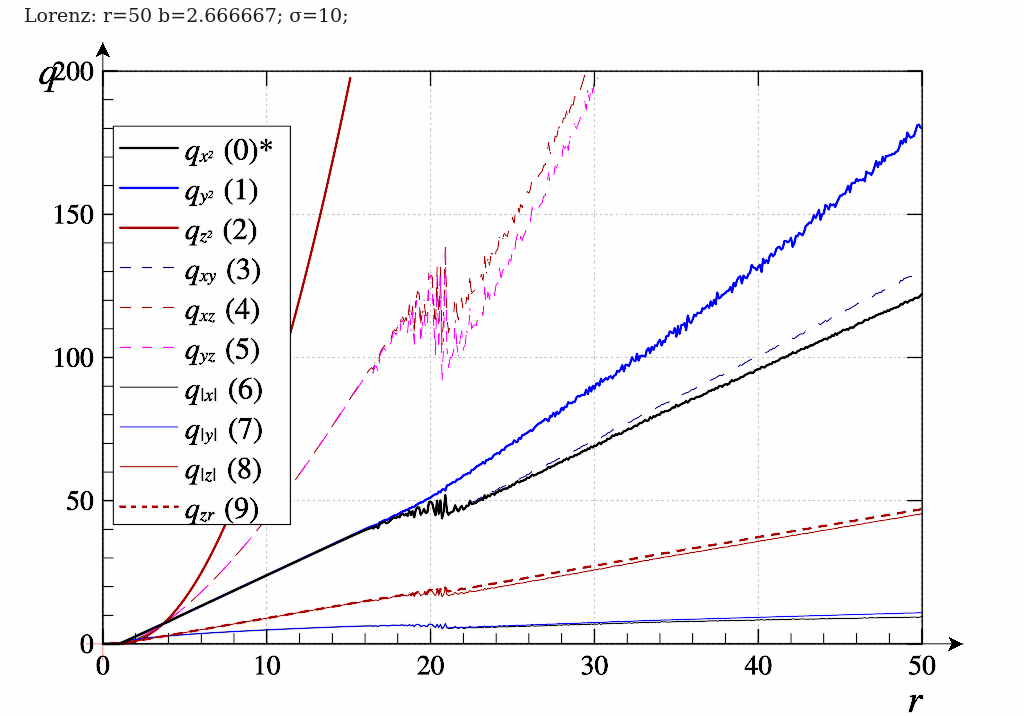
\includegraphics[width=0.7\textwidth]{p/cha/lor/lor_q-p_q_r.png} }
  \caption{Рассматриваемые критерии для системы Лоренца}
  \label{atu:f:lor_q}
\end{figure}

Анализ графиков позволяет сделать вывод, что практически все
рассмотренные виды критериев должны позволять построить
работоспособную систему идентификации. При этом,
большая часть графиков, в том числе и изначально
предложенный $q_{x^2}$, теряют монотонность
при переходе от режима затухающих колебаний к хаотическому,
что может помешать процессу идентификации вблизи этой точки.
Тем не менее, режим затухающих колебаний не представляет
практического интереса, и этим недостатком можно пренебречь.
Этого недостатка лишён критерий $q_{y^2}$, однако,
в рассматриваемых физических задачах значение
$y(t)$ наблюдать сложнее.
Критерий $q_{z^2}$ имеет явно выраженную параболическую форму,
а критерии $q_{zr}$ и $q_{|z|}$ также являются потенциальными кандидатами
в применимые критерии.
Критерии вида $q_{xy}$, $q_{xz}$ и $q_{yz}$
мало пригодны из-за высокого уровня колебаний.
Спектры же сигналов $x(t)$, $y(t)$ и $z(t)$
имеют практически одинаковую структуру.
Поэтому, в дальнейших исследованиях ограничимся
критериями
$q_{x^2}$ и
$q_{y^2}$.

Следующая зависимость, необходимая для синтеза
системы идентификации -- $ \sigma_q(\tau_q) $
или же  $ \sigma_q(a_q) $ -- соотношение между
временем оценивания $\tau_q$ и среднеквадратичной
ошибкой измерения критерия.
Для моделирования непосредственных погрешностей измерения величин
$x(t)$ и $y(t)$ использовался шум с нормальным распределением
и параметрами $\sigma_w=0.5$ и $\tau_w=0.05$~\cite{atu_asau26}.
Для оценивания требуемой зависимости, для каждого
значения $\tau_q$ из заданного диапазона
проводилось $N=200$ процессов моделирования динамики системы,
и в случайный момент (достаточно далеко отстоящий от точки $t=0$ для исключения краевых эффектов)
проводилось измерение и запоминание выбранного критерия.
При этом, для усреднения величины $q$ использовалось 2 метода:
экспоненциальное сглаживание, вида (\ref{atu:eq:qlin}), и скользящее среднее~(\ref{atu:eq:moving_avarage}).
Полученные зависимости, обозначенные соответственно
$\sigma_{ql}$ и $\sigma_{qa}$, представлены на
рис.~\ref{atu:f:lor_qy2_tau} и~\ref{atu:f:lor_qx2_tau}.


\begin{figure}[ht!]
\begin{center}
  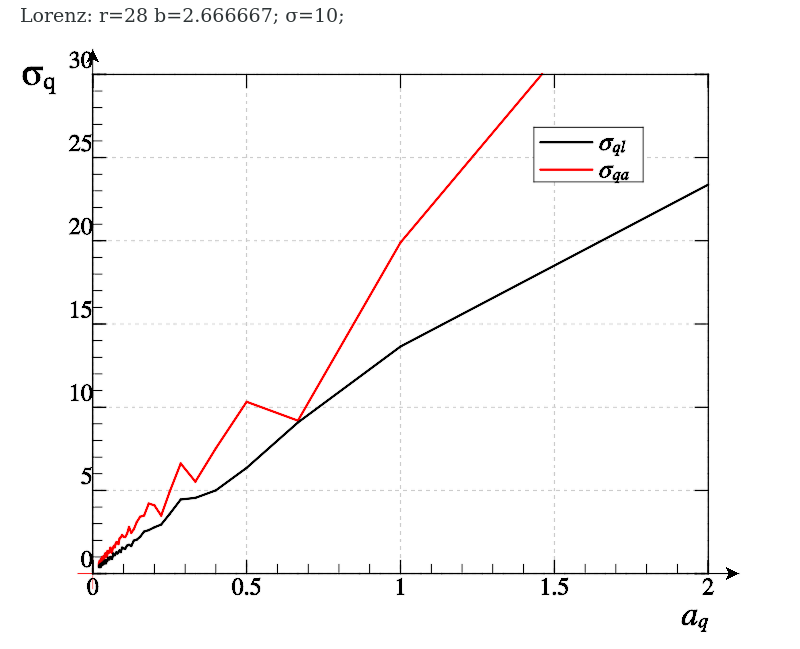
\includegraphics[width=0.49\textwidth]{p/cha/lor/lor_q_tau-p_aq_sd.png}
  \hfill
  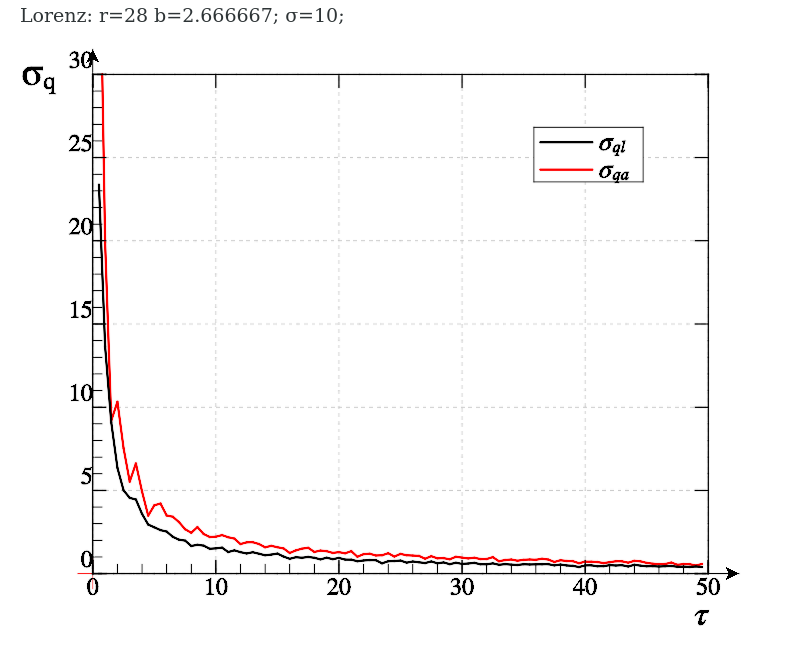
\includegraphics[width=0.49\textwidth]{p/cha/lor/lor_q_tau-p_tau_sd.png}
\end{center}
  \caption{Зависимости $\sigma_{q}(a_q)$ и $\sigma_{q}(\tau_q)$ для системы Лоренца, критерий  $q_{y^2}$}
\label{atu:f:lor_qy2_tau}
\end{figure}


\begin{figure}[ht!]
\begin{center}
  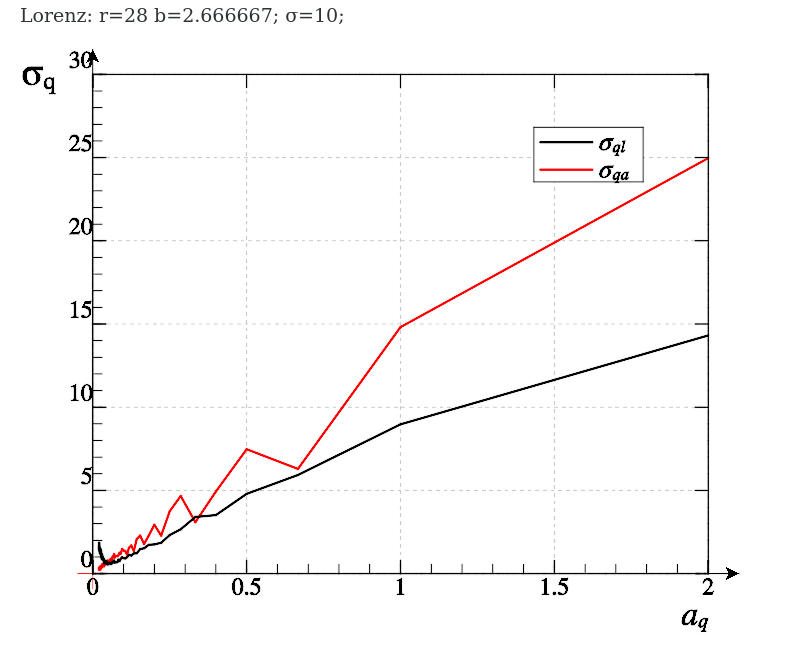
\includegraphics[width=0.49\textwidth]{p/cha/lor/lor_qx2_tau-p_aq_sd.png}
  \hfill
  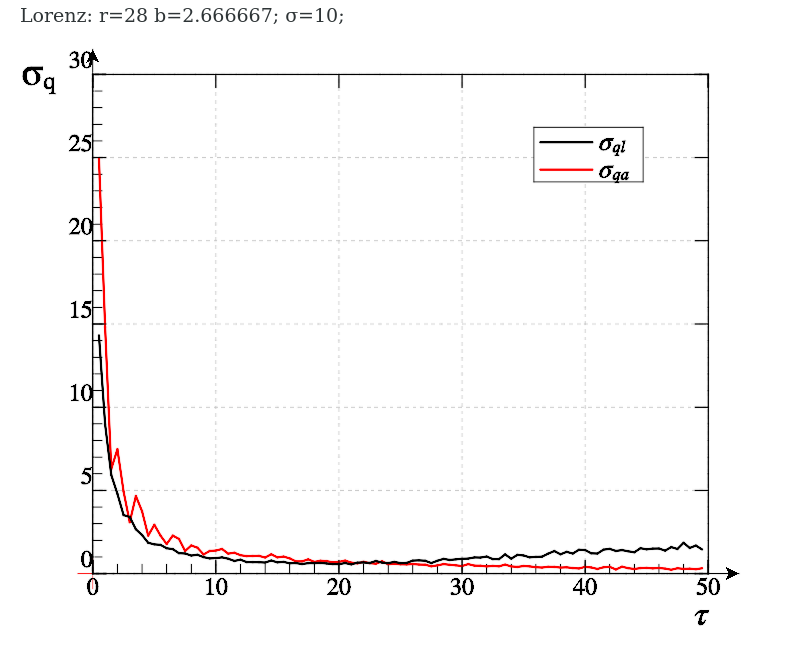
\includegraphics[width=0.49\textwidth]{p/cha/lor/lor_qx2_tau-p_tau_sd.png}
\end{center}
  \caption{Зависимости $\sigma_{q}(a_q)$ и $\sigma_{q}(\tau_q)$ для системы Лоренца, критерий $q_{x^2}$}
\label{atu:f:lor_qx2_tau}
\end{figure}

Анализ полученных зависимостей позволяет сделать
несколько выводов. Прежде всего, для рассматриваемой системы
результат усреднения с помощью значительно более затратного
в реализации метода скользящего среднего практически везде
уступает более простому методу. Таким образом,
при реализации методов идентификации в условиях с ограниченным ресурсами,
например на микроконтроллерной платформе в реальном времени,
нет смысла реализовывать ресурсоёмкоё скользящее среднее.
Далее, сам вид зависимости оказался достаточно простым:
$ \sigma_q \sim q a_q $ или же
$ \frac{\sigma_q \tau_q}{q} \approx \mathrm{const}$.

% }}}2


\subsection{Тестовая задача идентификации для системы Лоренца}  % {{{2

В соответствии с полученными данными, и используя
предложения~(\ref{atu:eq:po_t_sign}) и~(\ref{atu:eq:po_t_sin}),
определим тестовую задачу следующим образом:
\[
  p(t) \in [20, 60],
\]
%
\begin{equation}
  r_o(t) = p_o(t) = p_0 +  U_{p} \sign \sin( \omega_{p} t ),
  \label{atu:eq:lor_po_t_sign}
\end{equation}
%
%
\begin{equation}
  r_o(t) = p_o(t) = p_0 +  U_{p} \sin( \omega_{p} t ),
  \label{atu:eq:lor_po_t_sin}
\end{equation}
%
где:
$p_0 = 37$, $U_p=12$, $\omega_p=0.09$.

В качестве точки отсчёта рассмотрим применение уже рассмотрено в работе \Cmt{[atu-phd]}
метода с одним агентом, управляющим двумя моделями,
и использующий два УГПК и интегратором для определения динамики агента.
Для возможности применения данного метода к системе динамического хаоса
как объект, так и модели были дополнены блоками оценивания критерия $q_{x^2}$.
Таким образом, согласно ведённой классификации,
метод получает обозначение
``Fl2nlosdlcA.$q_{x^2}$''.

Прежде всего, рассмотрим процессы идентификации параметра $r$
системы Лоренца данным методом. Типичные результаты моделирования
приведены на рис.~(\ref{atu:f:lor_id_Fl2nlosdlcA_wp009}).

\begin{figure}[ht!]
  \centerline{
    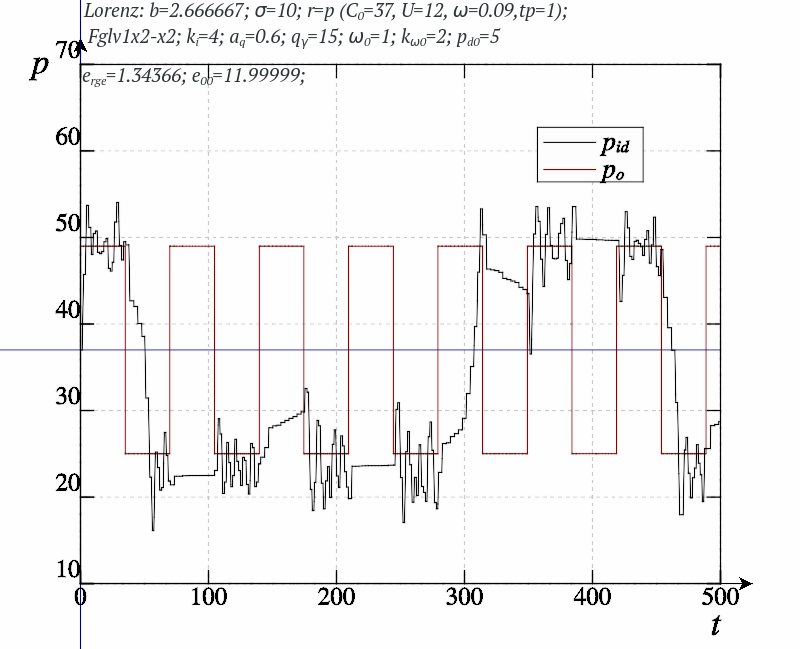
\includegraphics[width=0.49\textwidth]{p/cha/lor/Fl2nlosdlcA/Fl2nlosdlcA-p_xz_1_wp009.png}
    \hfill
    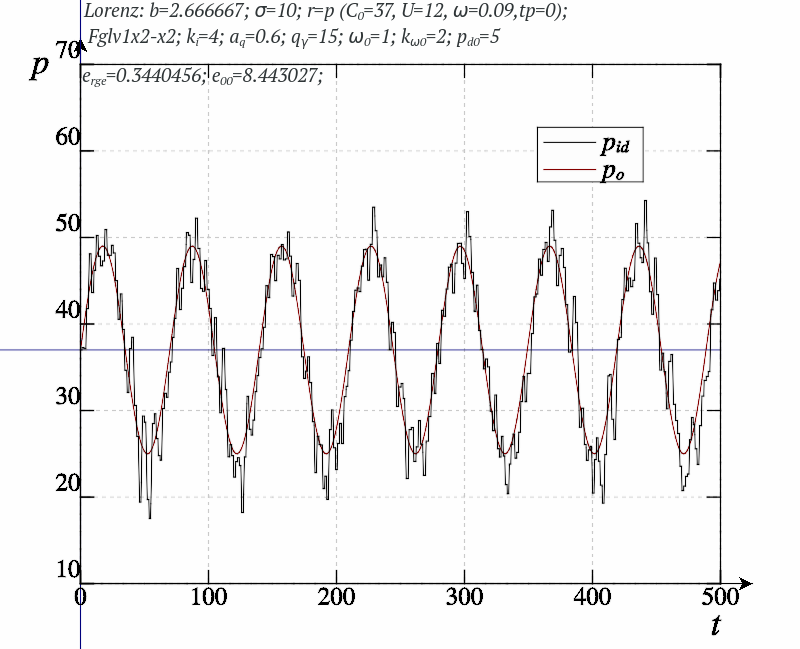
\includegraphics[width=0.49\textwidth]{p/cha/lor/Fl2nlosdlcA/Fl2nlosdlcA-p_xz_0_wp009.png}
  }
  \caption{Процесс идентификации параметра ``$r$'' системы Лоренца методом Fl2nlosdlcA.$q_{x^2}$ при условиях~(\ref{atu:eq:lor_po_t_sign}) и (\ref{atu:eq:lor_po_t_sin})}
  \label{atu:f:lor_id_Fl2nlosdlcA_wp009}
\end{figure}

Как видно из графиков процессов идентификации,
при заданных условиях и
при достаточно плавном изменении параметров
(\ref{atu:eq:lor_po_t_sin}) процесс идентификации приводит
к положительному результату. Если же значения параметра изменяются
скачкообразно~(\ref{atu:eq:lor_po_t_sign}),
то процесс поиска нарушается -- система просто не успевает
отреагировать на такие изменения. Попытки уменьшить
время реакции за счёт изменения соответствующих
параметров ($a_q$, $k_\omega$, $k_i$) приводят к полному нарушению
процесса поиска. С другой стороны, уменьшение чувствительности
(увеличение $q_\gamma$) даёт возможность восстановить
работоспособность процесса идентификации ценой
значительного увеличения ошибки.

Для проверки тезиса о том, что в данном случае играет роль
именно динамика изменения $p_o(t)$, снизим частоту $\omega_p$ до $0.03$
и проведём моделирование при тех же значениях
всех остальных параметров. Результаты приведены на рис.~\ref{atu:f:lor_id_Fl2nlosdlcA_003}.

\begin{figure}[ht!]
  \centerline{
    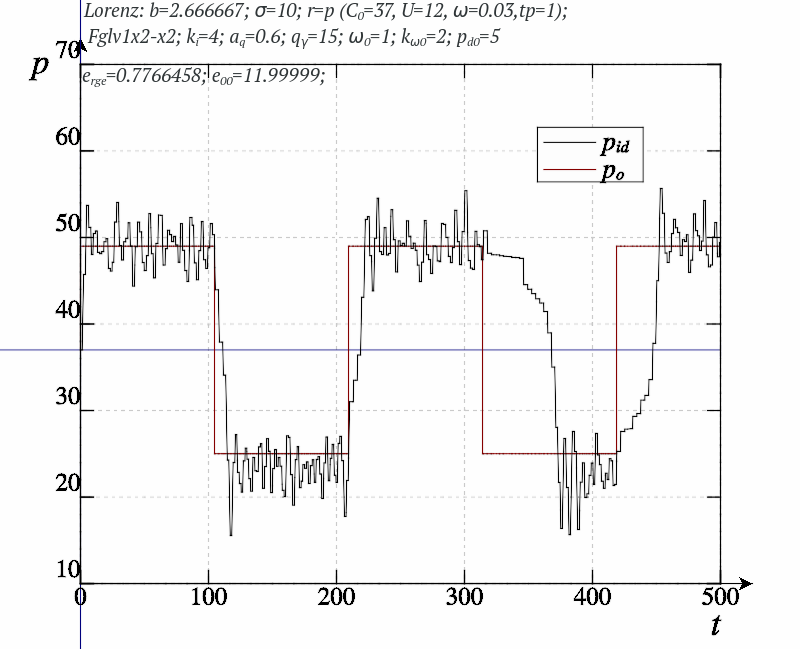
\includegraphics[width=0.49\textwidth]{p/cha/lor/Fl2nlosdlcA/Fl2nlosdlcA-p_xz_1_wp003.png}
    \hfill
    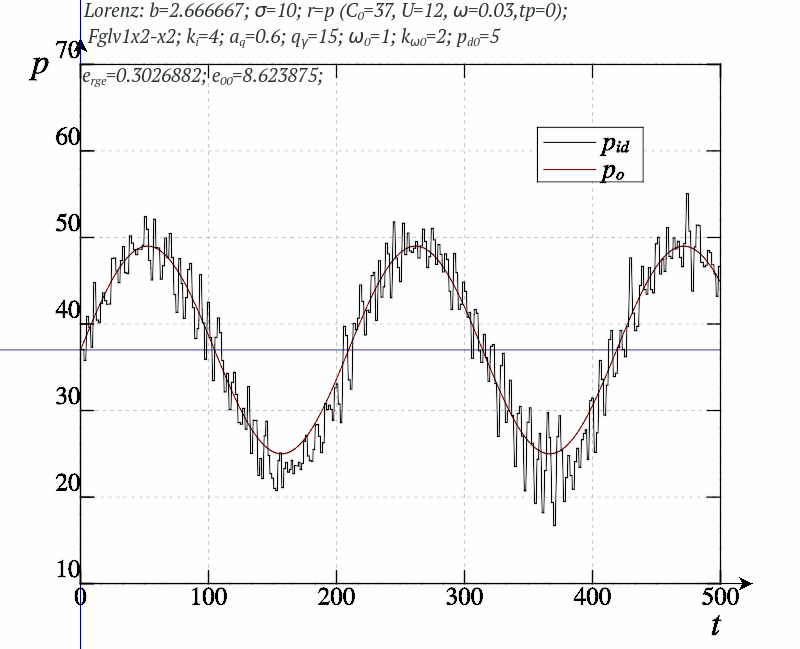
\includegraphics[width=0.49\textwidth]{p/cha/lor/Fl2nlosdlcA/Fl2nlosdlcA-p_xz_0_wp003.png}
  }
  \caption{Процесс идентификации параметра ``$r$'' системы Лоренца методом Fl2nlosdlcA.$q_{x^2}$ при $\omega_p=0.03$}
  \label{atu:f:lor_id_Fl2nlosdlcA_003}
\end{figure}

Как и следовало ожидать, при меньшем значении $\omega_p$
оба графика подтверждают работоспособность системы идентификации.

Для оценивания границ применимости метода с одним агентом
и двумя моделями построим зависимости
$\overline{e}_{rge}(\omega_p)$~(рис.~\ref{atu:f:lor_Fl2nlosdlcA_e_omega_p}).

\begin{figure}[ht!]
  \centerline{
    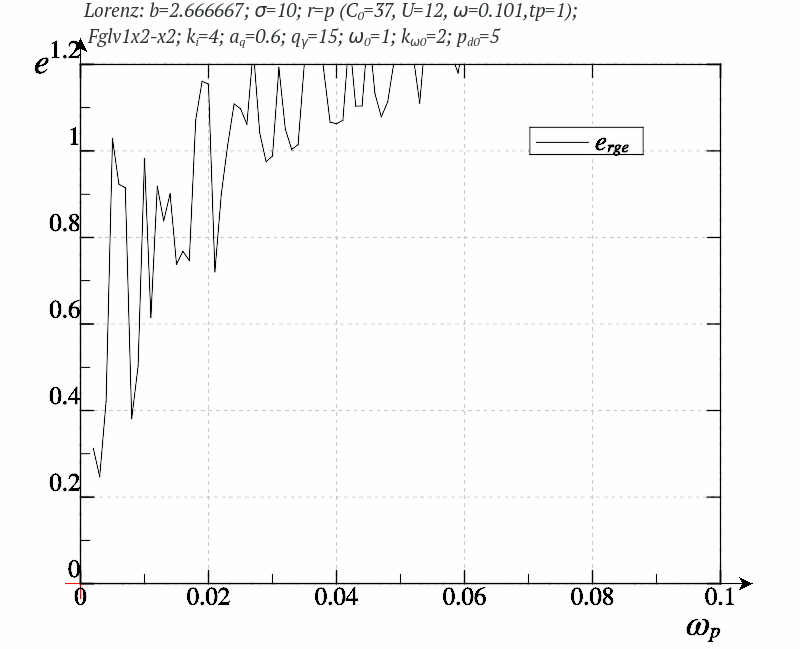
\includegraphics[width=0.49\textwidth]{p/cha/lor/Fl2nlosdlcA/Fl2nlosdlcA-p_omega_p_e_1.png}
    \hfill
    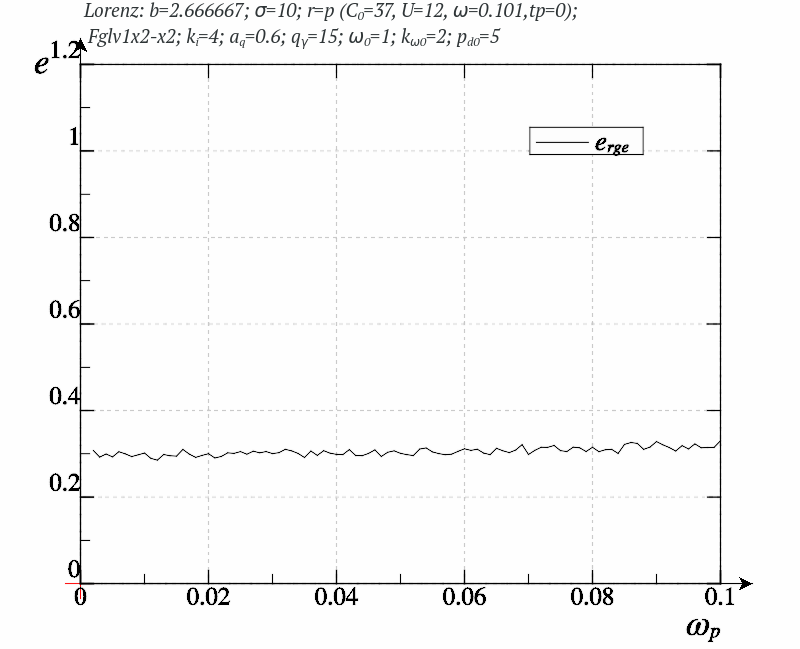
\includegraphics[width=0.49\textwidth]{p/cha/lor/Fl2nlosdlcA/Fl2nlosdlcA-p_omega_p_e_0.png}
  }
  \caption{Зависимости $\overline{e}_{rge}(\omega_p)$ при идентификации системы Лоренца методом Fl2nlosdlcA.$q_{x^2}$}
  \label{atu:f:lor_Fl2nlosdlcA_e_omega_p}
\end{figure}

Совершенно очевидно, что рассматриваемая система идентификации
имеет очень ограниченный диапазон применимости при условии~(\ref{atu:eq:lor_po_t_sign}).
Условие~(\ref{atu:eq:lor_po_t_sin}) не налагает таких жёстких ограничений.
Однако, рассмотрев эту же зависимость в другом масштабе~(рис.~\ref{atu:f:lor_Fl2nlosdlcA_e_omega_p_wide}),
мы увидим, что ограничение всё же присутствует.

\begin{figure}[ht!]
  \centerline{
    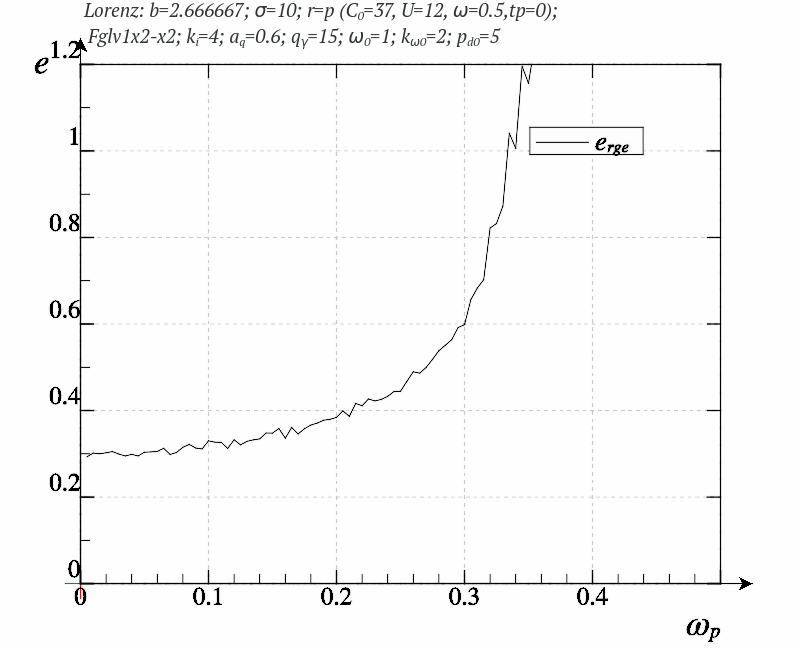
\includegraphics[width=0.49\textwidth]{p/cha/lor/Fl2nlosdlcA/Fl2nlosdlcA-p_omega_p_e_0_wide.png}
  }
  \caption{Зависимость $\overline{e}_{rge}(\omega_p)$ при идентификации системы Лоренца методом Fl2nlosdlcA.$q_{x^2}$}
  \label{atu:f:lor_Fl2nlosdlcA_e_omega_p_wide}
\end{figure}

Так как основным недостатком рассмотренного метода является
ограниченная реакция на резкое изменение параметра,
то имеет смысл выдвинуть предположение,
что использование в системе идентификации нескольких агентов,
распределённых на пространстве параметров, может
скомпенсировать данный недостаток.


Для сравнения были выбраны три группы мультимодельных методов идентификации~\cite{atu_ISDMCI2015,atu_asau26}:
ql3ruonAAF.$q_{x^2}$,
ql3ruonAAF.$q_{y^2}$ и
Fq3zlovnAAF.$q_{x^2}$.
Символы ``A'' в каждом из
обозначений~(см.~стр.~\pageref{atu:id_classification})
индицируют, что проверяются
% все
несколько способов определения $p_\mathrm{id}$.
Количество агентов и способ их группировки (5.3) были выбраны
одинаковыми для корректного сравнения различных походов.


На рис.~\ref{atu:f:lor_id_ql3ruonAAF.q_x2_sign} представлены результаты идентификации
методом ql3ruonAAF.$q_{x^2}$, при этом на левом графике представлена
динамика перемещения каждой из подвижных моделей,
а на правом -- 4 способа определения $p_{id}(t)$:
$p_{gc}$, $p_{lc}$, $p_{ge}$ и $p_{le}$.
В первую очередь, следует отметить общую работоспособность
методов, и правильную динамику каждой из моделей.


Сравнивая результаты различных способов определения
$p_{id}$ как визуально, так и численно, можно сделать
вывод, что худшие результаты демонстрирует $p_{ee}$.
Этого и следовало ожидать, так как это подход, в первую очередь,
был предназначен для методов идентификации, использующих
функцию качества для определения $p_e$.
Также, совершенно ожидаемо, лучшие результаты продемонстрировал
подход $p_{ee}$. Также, при искусственных ограничения
$v_f=0$ и $q_\gamma=0.1$ были получены величины,
характеризующие качество идентификации для неподвижных агентов:
$\overline{e}_{bc}=9.85$
и
$\overline{e}_{be}=7.09$, что свидетельствует
о оправданности как перемещения агентов,
так и использовании величин $p_e$ для определения $p_{id}$.



\begin{figure}[ht!]
  \centerline{
    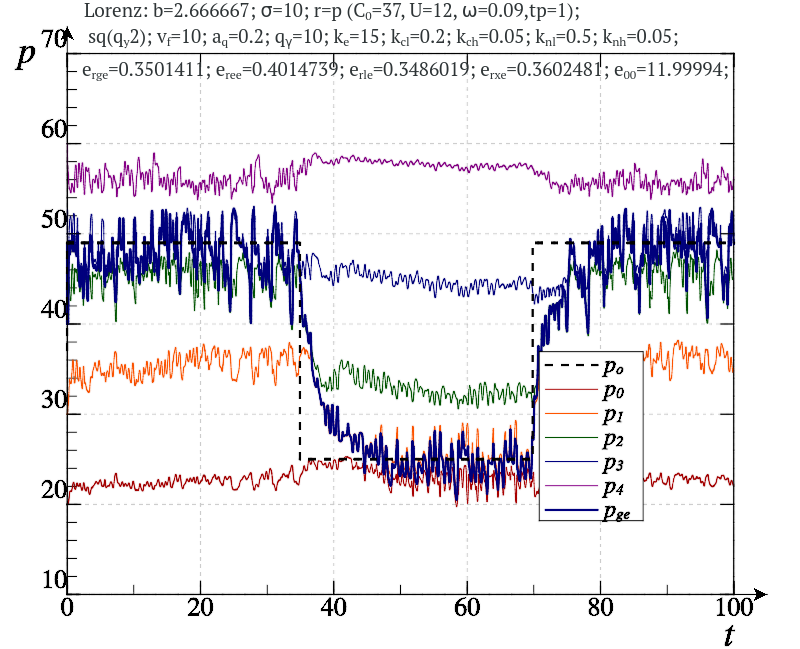
\includegraphics[width=0.49\textwidth]{p/cha/lor/ql3ruonAAF/lor_ql3ruonAAF_qy2-p_t_pi_sign.png}
    \hfill
    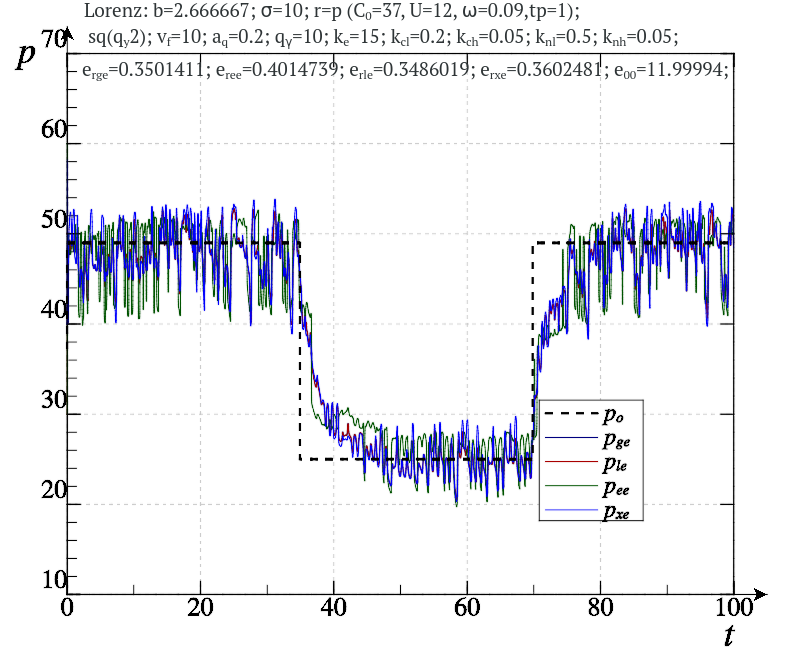
\includegraphics[width=0.49\textwidth]{p/cha/lor/ql3ruonAAF/lor_ql3ruonAAF_qy2-p_t_pz_sign.png}
  }
  \caption{Процесс идентификации параметра ``$r$'' системы Лоренца методом ql3ruonAAF.$q_{x^2}$ при условии~(\ref{atu:eq:lor_po_t_sign})}
  \label{atu:f:lor_id_ql3ruonAAF.q_x2_sign}
\end{figure}


На рис.~\ref{atu:f:lor_id_ql3ruonAAF.q_x2_sin} представлены аналогичные результаты,
но при условии плавного изменение значения параметра объекта. Как и следовало ожидать,
как абсолютные, так и относительные значения ошибок идентификации в данном случае заметно
меньше, при сохранении общей картины.
При этом
$\overline{e}_{bc}=7.80$
и
$\overline{e}_{be}=5.24$.


\begin{figure}[ht!]
  \centerline{
    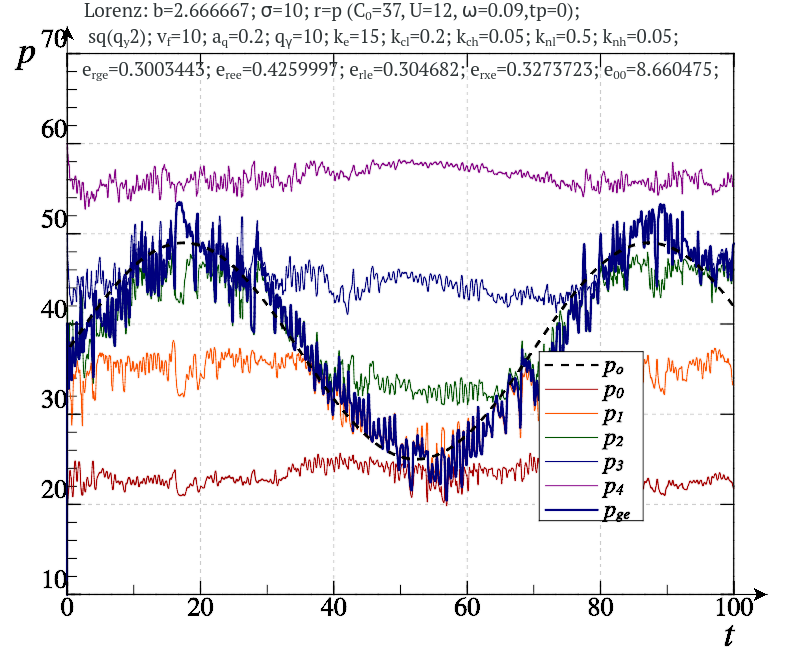
\includegraphics[width=0.49\textwidth]{p/cha/lor/ql3ruonAAF/lor_ql3ruonAAF_qy2-p_t_pi_sin.png}
    \hfill
    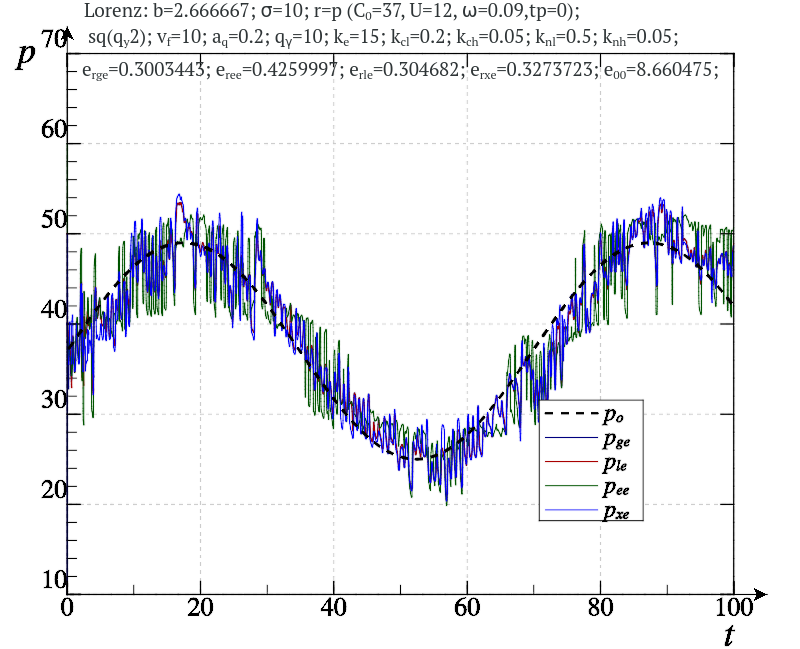
\includegraphics[width=0.49\textwidth]{p/cha/lor/ql3ruonAAF/lor_ql3ruonAAF_qy2-p_t_pz_sin.png}
  }
  \caption{Процесс идентификации параметра ``$r$'' системы Лоренца методом ql3ruonAAF.$q_{x^2}$ при условии~(\ref{atu:eq:lor_po_t_sin})}
  \label{atu:f:lor_id_ql3ruonAAF.q_x2_sin}
\end{figure}


На рис.~\ref{atu:f:lor_id_ql3ruonAAF.q_y2_sign} представлены результаты
полученные методом ql3ruonAAF.$q_{y^2}$,
отличающего от предыдущего только видом использованного критерия.
При этом
$\overline{e}_{bc}=10.85$
и
$\overline{e}_{be}=7.73$.

\begin{figure}[ht!]
  \centerline{
    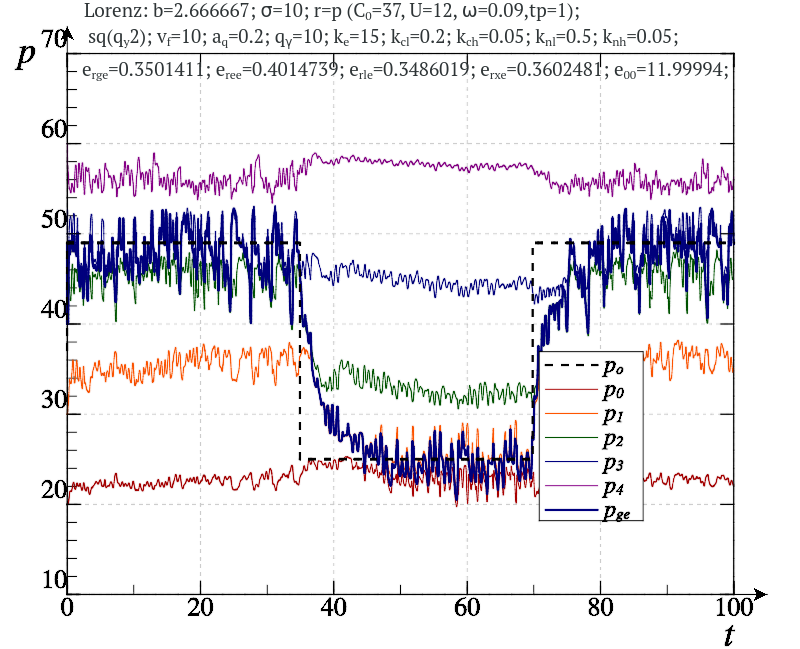
\includegraphics[width=0.49\textwidth]{p/cha/lor/ql3ruonAAF/lor_ql3ruonAAF_qy2-p_t_pi_sign.png}
    \hfill
    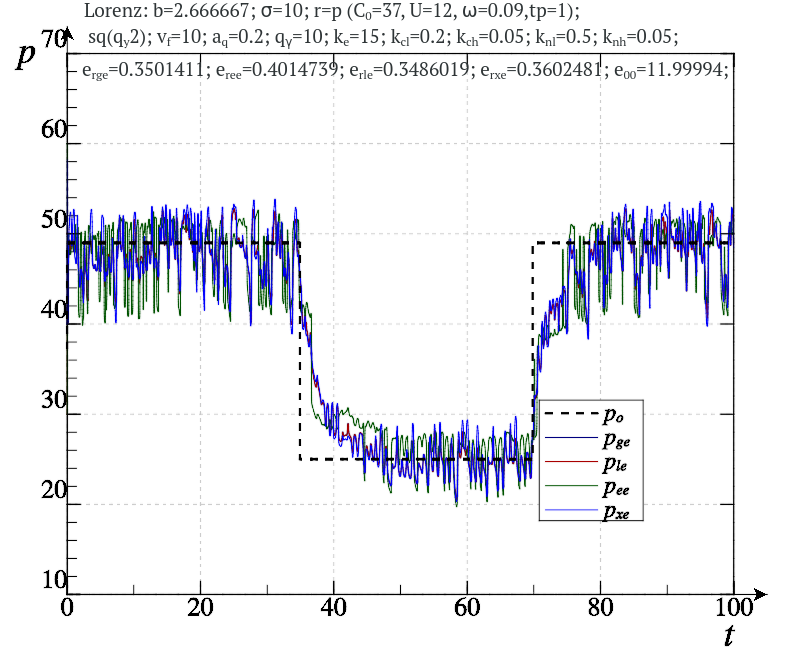
\includegraphics[width=0.49\textwidth]{p/cha/lor/ql3ruonAAF/lor_ql3ruonAAF_qy2-p_t_pz_sign.png}
  }
  \caption{Процесс идентификации параметра ``$r$'' системы Лоренца методом ql3ruonAAF.$q_{y^2}$ при условии~(\ref{atu:eq:lor_po_t_sign})}
  \label{atu:f:lor_id_ql3ruonAAF.q_y2_sign}
\end{figure}


На рис.~\ref{atu:f:lor_id_ql3ruonAAF.q_y2_sin} представлены аналогичные результаты,
только при условии (\ref{atu:eq:lor_po_t_sin}).
При этом
$\overline{e}_{bc}=8.09$
и
$\overline{e}_{be}=5.46$.


\begin{figure}[ht!]
  \centerline{
    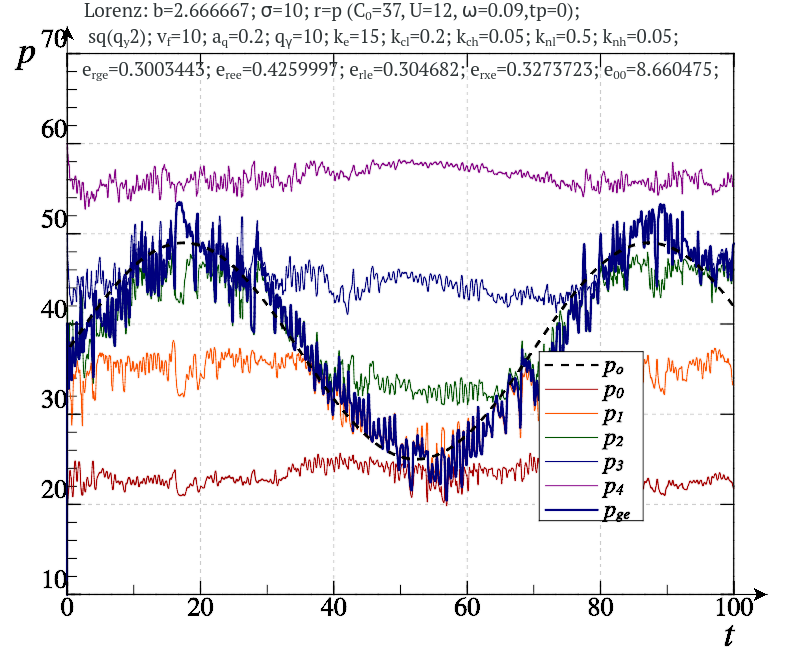
\includegraphics[width=0.49\textwidth]{p/cha/lor/ql3ruonAAF/lor_ql3ruonAAF_qy2-p_t_pi_sin.png}
    \hfill
    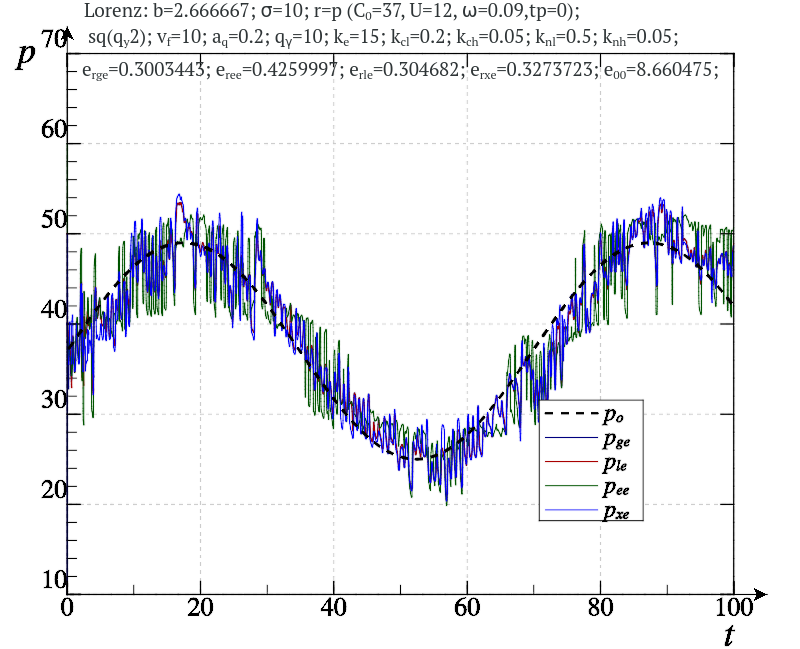
\includegraphics[width=0.49\textwidth]{p/cha/lor/ql3ruonAAF/lor_ql3ruonAAF_qy2-p_t_pz_sin.png}
  }
  \caption{Процесс идентификации параметра ``$r$'' системы Лоренца методом ql3ruonAAF.$q_{x^2}$ при условии~(\ref{atu:eq:lor_po_t_sin})}
  \label{atu:f:lor_id_ql3ruonAAF.q_y2_sin}
\end{figure}

Также важным результатом является тот факт, что, по сравнению с одноагентным методом,
система идентификации не теряет работоспособности
при резких изменениях параметра. Зависимости $\overline{e}_{rge}(\omega_p)$
для данного семейства методов приведены на рис.~\ref{atu:f:lor_ql3ruonAAF_e_omega_p}.


\begin{figure}[ht!]
  \centerline{
    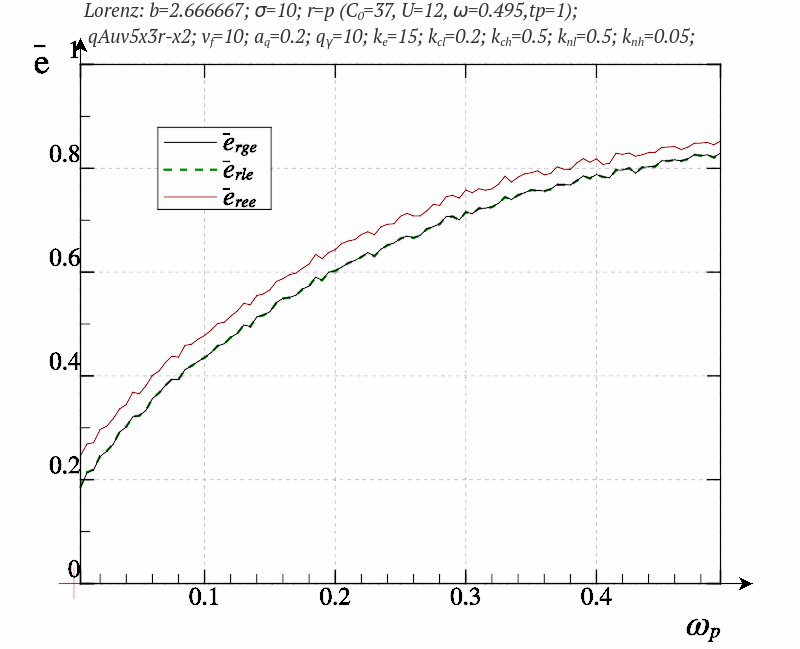
\includegraphics[width=0.49\textwidth]{p/cha/lor/ql3ruonAAF/lor_ql3ruonAAF_qx2-p_omega_p_e_sign.png}
    \hfill
    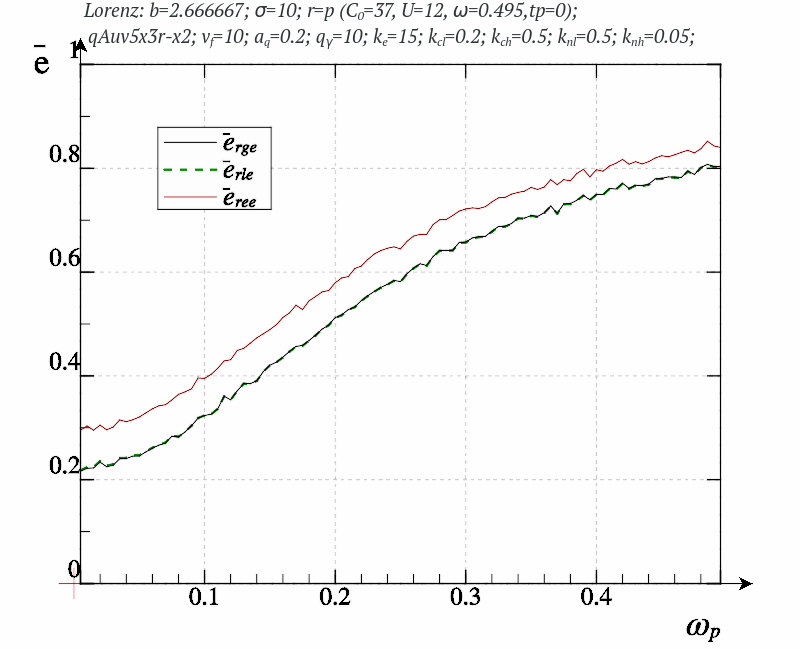
\includegraphics[width=0.49\textwidth]{p/cha/lor/ql3ruonAAF/lor_ql3ruonAAF_qx2-p_omega_p_e_sin.png}
  }
  \caption{Зависимости $\overline{e}_{rge}(\omega_p)$ при идентификации системы Лоренца методом ql3ruonAAF.$q_{x^2}$}
  \label{atu:f:lor_ql3ruonAAF_e_omega_p}
\end{figure}

Сравнивавшая получившиеся зависимости с аналогичными для одноагентого метода (рис.~\ref{atu:f:lor_Fl2nlosdlcA_e_omega_p}),
можно с уверенностью констатировать,
что применение мультиагентного подхода здесь полностью оправданно.
Во-первых, допустимый диапазон $\omega_p$ расширяется как минимум на порядок. % TODO: limit?
С другой стороны, в этом случае нет принципиальной разницы между
условиями~(\ref{atu:eq:lor_po_t_sign}) и (\ref{atu:eq:lor_po_t_sin}),
что также является несомненным преимуществом.




Сравнивая результаты, представленные на рис.~\ref{atu:f:lor_id_ql3ruonAAF.q_x2_sign}--\ref{atu:f:lor_id_ql3ruonAAF.q_y2_sin}
можно сделать следующие выводы:

\begin{itemize}

  \item
    Динамика систем идентификации при использовании критериев $q_{x^2}$ и $q_{y^2}$
    практически совпадает.

  \item
    Применение критерия  $q_{y^2}$ в данном конкретном случае позволяет
    меньшую ошибку идентификации, но на настолько,
    чтобы можно было говорить о существенной разнице.

  \item
    Во всех рассмотренных случаях оправданными были и применение нескольких агентов,
    и их смещение в процессе поиска, и определение с помощью $p_e$
    каждого из агентов.

\end{itemize}

Рассмотрим процесс идентификации этой же системы, при тех же условиях,
но семейством методов, основанных на применении функции качества,
а именно Fq3zlovnAAF.$q_{x^2}$

Процесс идентификации при условии~(\ref{atu:eq:lor_po_t_sign})
представлен на рис.~\ref{atu:f:lor_id_Fq3zlovnAAF.q_x2_sign}.
В первую очередь следует отметить большую подвижность
агентов, вплоть до искусственного ограничения подвижности
большей части моделей. С одной стороны, это несколько уменьшает
быстродействие системы при резких изменениях параметра,
с другой -- обеспечивает достаточное смещение ``дальних'' агентов,
что, в какой-то мере, компенсирует возможные ошибки в настройке системы.
Величина $\overline{e}_{bc}=10.84$ имеет примерно такое же значение,
как и предыдущих случаях,
а $\overline{e}_{be}$ в данных условиях не применима.

\begin{figure}[ht!]
  \centerline{
    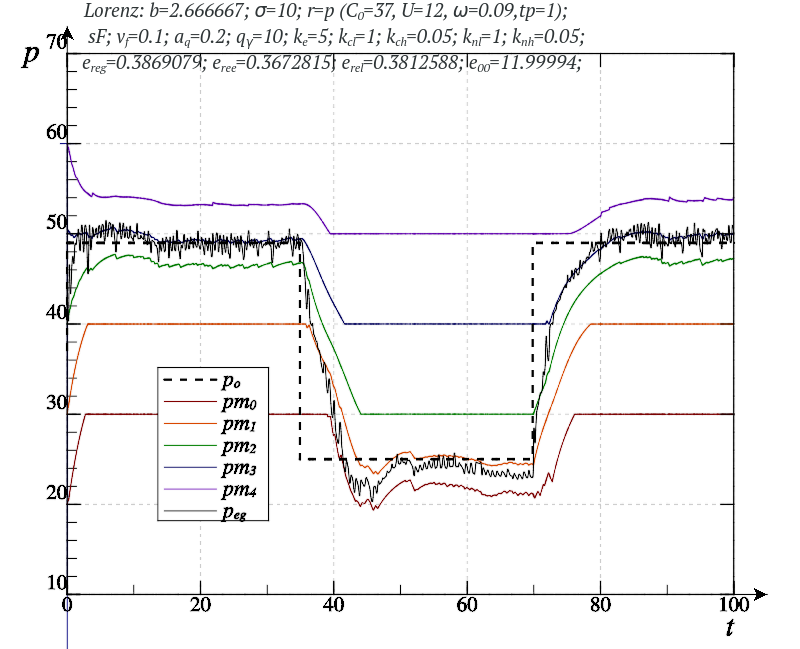
\includegraphics[width=0.49\textwidth]{p/cha/lor/Fq3zlovnAAF/lor_Fq3zlovnAAF_qx2-pl_n_sign.png}
    \hfill
    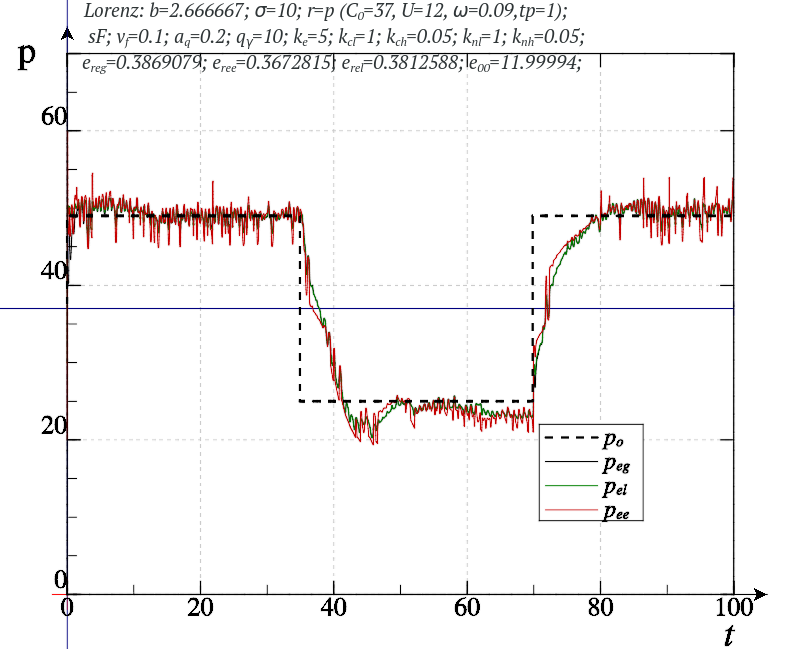
\includegraphics[width=0.49\textwidth]{p/cha/lor/Fq3zlovnAAF/lor_Fq3zlovnAAF_qx2-p_p_sign.png}
  }
  \caption{Процесс идентификации параметра ``$r$'' системы Лоренца методом Fq3zlovnAAF.$q_{x^2}$ при условии~(\ref{atu:eq:lor_po_t_sign})}
  \label{atu:f:lor_id_Fq3zlovnAAF.q_x2_sign}
\end{figure}

На рис.~\ref{atu:f:lor_id_Fq3zlovnAAF.q_x2_sin}
процесс идентификации при условии~(\ref{atu:eq:lor_po_t_sin}).
Величина $\overline{e}_{bc}=7.95$ не выбивается из общего ряда,
и общая картина имеет ожидаемый вид.

\begin{figure}[ht!]
  \centerline{
    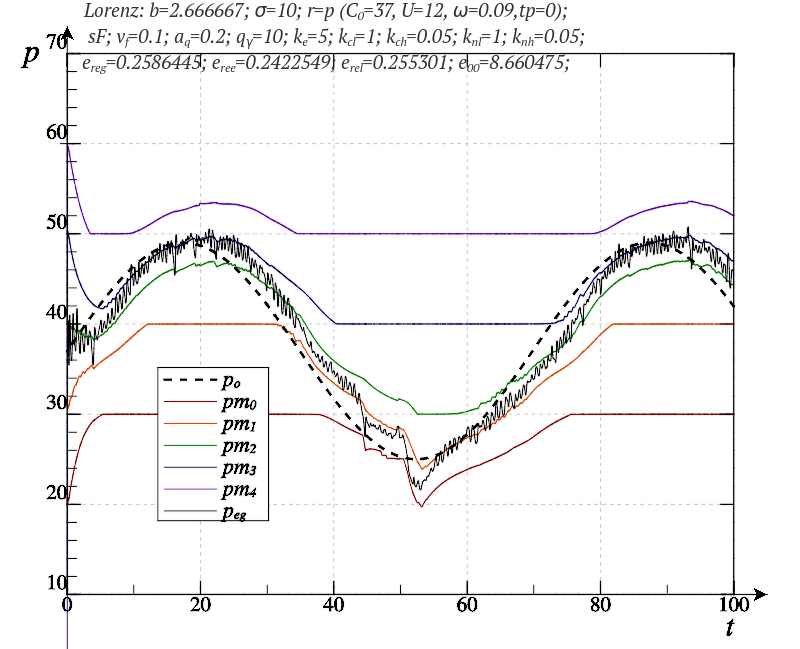
\includegraphics[width=0.49\textwidth]{p/cha/lor/Fq3zlovnAAF/lor_Fq3zlovnAAF_qx2-pl_n_sin.png}
    \hfill
    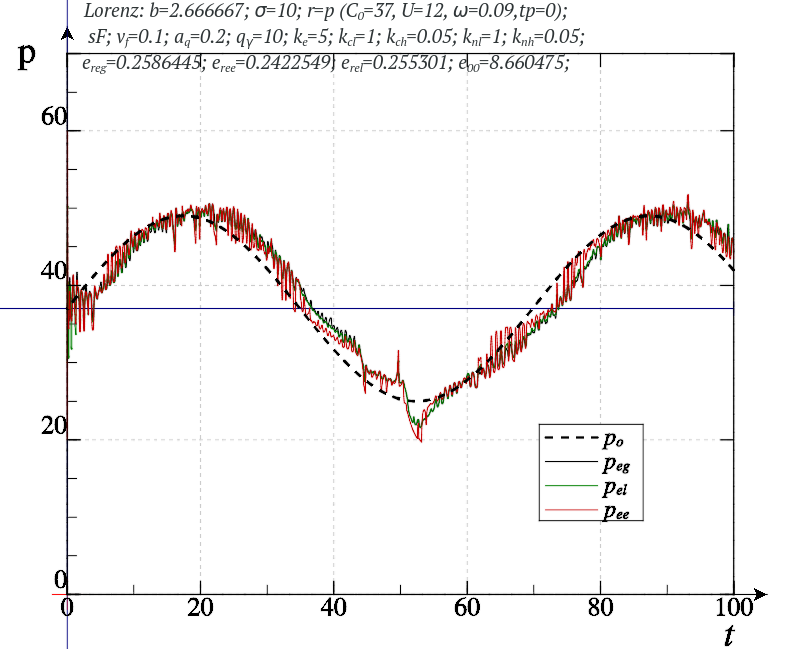
\includegraphics[width=0.49\textwidth]{p/cha/lor/Fq3zlovnAAF/lor_Fq3zlovnAAF_qx2-p_p_sin.png}
  }
  \caption{Процесс идентификации параметра ``$r$'' системы Лоренца методом Fq3zlovnAAF.$q_{x^2}$ при условии~(\ref{atu:eq:lor_po_t_sin})}
  \label{atu:f:lor_id_Fq3zlovnAAF.q_x2_sin}
\end{figure}

Также следует отметить, что данный метод, аналогично предыдущему,
проявляет работоспособность при резких изменениях параметра.
Построим зависимости
$\overline{e}_{rge}(\omega_p)$ (рис.~\ref{atu:f:lor_Fq3zlovnAAF_e_omega_p}).


\begin{figure}[ht!]
  \centerline{
    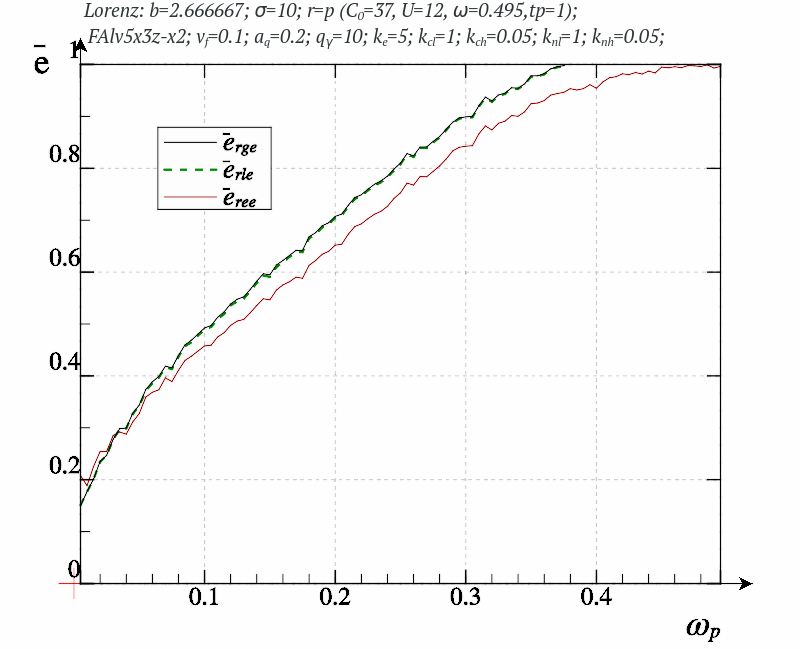
\includegraphics[width=0.49\textwidth]{p/cha/lor/Fq3zlovnAAF/lor_Fq3zlovnAAF_qx2-p_omega_p_e_sign.png}
    \hfill
    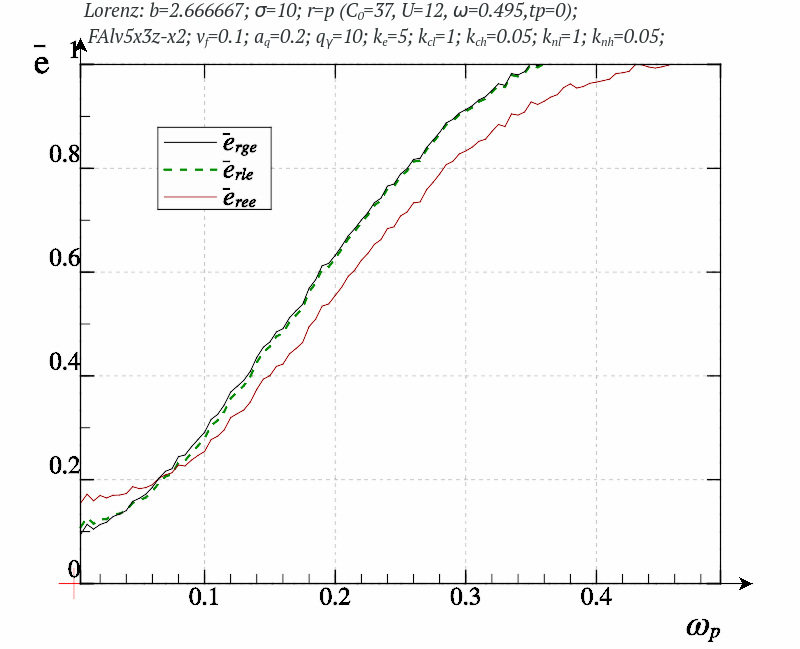
\includegraphics[width=0.49\textwidth]{p/cha/lor/Fq3zlovnAAF/lor_Fq3zlovnAAF_qx2-p_omega_p_e_sin.png}
  }
  \caption{Зависимости $\overline{e}_{rge}(\omega_p)$ при идентификации системы Лоренца методом Fblvd1.2.$q_{x^2}$}
  \label{atu:f:lor_Fq3zlovnAAF_e_omega_p}
\end{figure}

Вид этих зависимостей аналогичен таковым для предыдущего метода,
хотя рабочий диапазон по $\omega_p$ незначительно уже.
Таким образом, применение мультимодельного подхода
оправданно, по крайней мере с этой точки трения,
вне зависимости от того, какую величину, $q$ или $F$
используют агенты для определения $p_e$.

% }}}2


% ----------------------------------------- id_params -------------------------------

\subsection{Влияние параметров системы идентификации на ошибку идентификации для системы Лоренца}  % {{{2

Рассмотрим влияние параметров системы идентификации на
процесс идентификации и, следовательно, на её качество~\cite{atu_ISDMCI2014}.
Для этого будем варьировать каждый из существенных
параметров и строить зависимости $\overline{e}$
для каждого из рассмотренных методов.

В первую очередь рассмотрим влияние параметра
$a_q$, определяющего характерное время усреднения.

На рис.~\ref{atu:f:lor_a_q_ql3ruonAAF.q_x2} представлены зависимости
усреднённых ошибок идентификации системы Лоренца от $a_q$ при использовании метода ql3ruonAAF.$q_{x^2}$.
Достаточно очевидно, что форма кривых с явным экстремумом обусловлена
влияниями противоборствующих факторов. При больших значениях $a_q$,
и, следовательно, малом времени усреднения $\tau_q$,
слишком сильно влияние хаотической динамики, что бы можно было бы
проводить успешную идентификацию. С другой стороны,
при слишком малых значениях $a_q$, время оценивание критерия настолько большое,
что система идентификации не успевает отслеживать изменение параметра.
Этот тезис подтверждается тем фактом, что при более плавном изменении параметра
(\ref{atu:eq:lor_po_t_sin})
минимум ошибок достигается при меньших значениях $a_q$.

\begin{figure}[ht!]
  \centerline{
    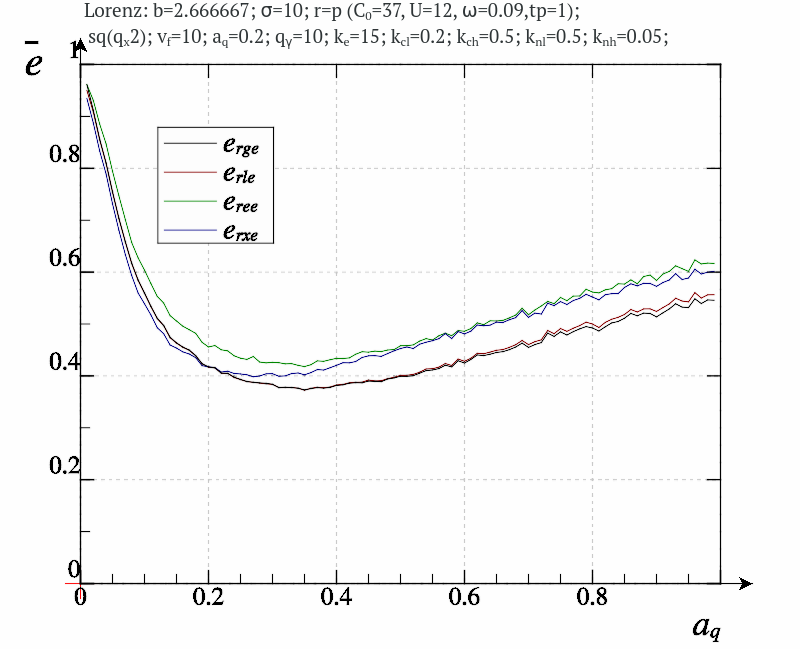
\includegraphics[width=0.49\textwidth]{p/cha/lor/ql3ruonAAF/lor_ql3ruonAAF_qx2-p_a_q_e_sign.png}
    \hfill
    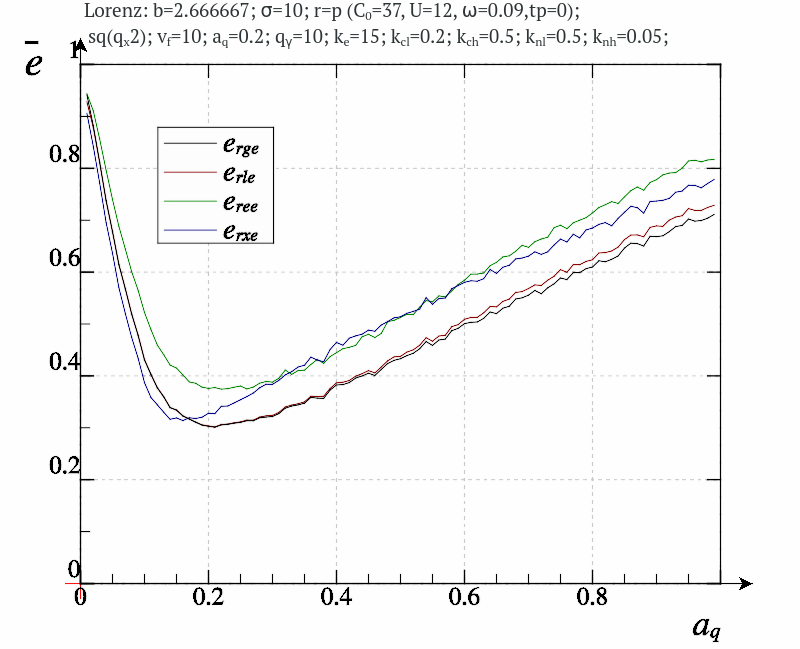
\includegraphics[width=0.49\textwidth]{p/cha/lor/ql3ruonAAF/lor_ql3ruonAAF_qx2-p_a_q_e_sin.png}
  }
  \caption{Зависимости $\overline{e}_{r*}(a_q)$ при идентификации системы Лоренца методом ql3ruonAAF.$q_{x^2}$
   при~(\ref{atu:eq:lor_po_t_sign}) и (\ref{atu:eq:lor_po_t_sin})}
  \label{atu:f:lor_a_q_ql3ruonAAF.q_x2}
\end{figure}


На рис.~\ref{atu:f:lor_a_q_ql3ruonAAF.q_y2} представлены зависимости
усреднённых ошибок идентификации системы Лоренца при использовании метода ql3ruonAAF.$q_{y^2}$.
Здесь ситуация существенно изменяется но сравнению с предыдущим случаем.
Положения экстремумов практически не изменились, но
при больших значениях $a_q$ начинает наблюдаться полное нарушение
процесса поиска. Таким образом, несмотря на то,
что в наилучших условиях критерий $q_{y^2}$ обеспечивает меньшую
ошибку идентификации, диапазон его применимости меньше. С учётом
того, момент нарушения поиска зависит и от формы $p_o(t)$,
а она в реальных задачах заранее не известна, использование этого критерия может
не быть оправданным.

\begin{figure}[ht!]
  \centerline{
    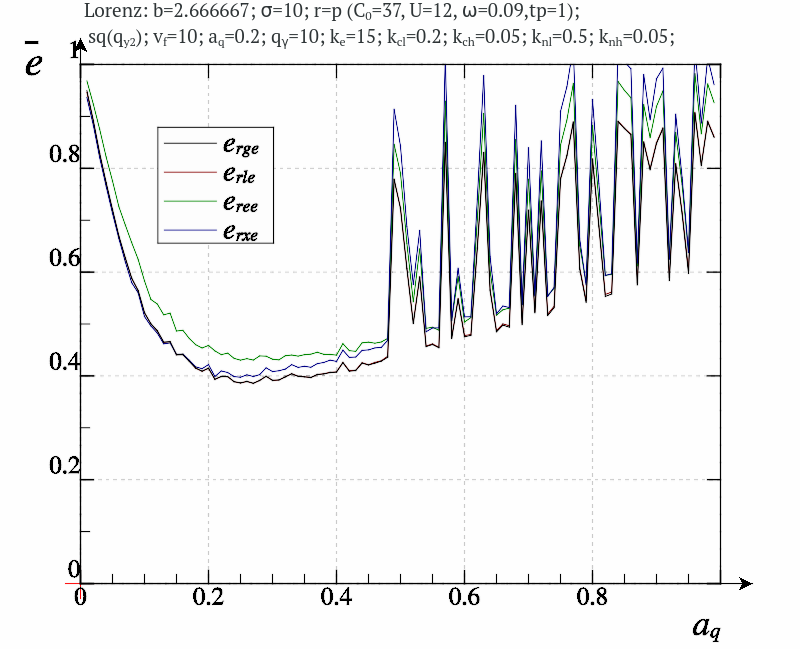
\includegraphics[width=0.49\textwidth]{p/cha/lor/ql3ruonAAF/lor_ql3ruonAAF_qy2-p_a_q_e_sign.png}
    \hfill
    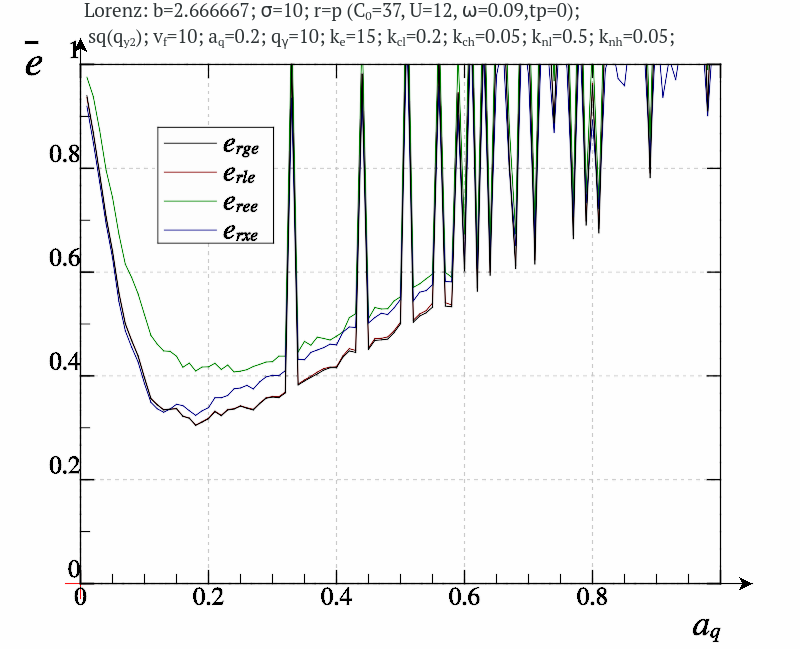
\includegraphics[width=0.49\textwidth]{p/cha/lor/ql3ruonAAF/lor_ql3ruonAAF_qy2-p_a_q_e_sin.png}
  }
  \caption{Зависимости $\overline{e}_{r*}(a_q)$ при идентификации системы Лоренца методом ql3ruonAAF.$q_{y^2}$
   при~(\ref{atu:eq:lor_po_t_sign}) и (\ref{atu:eq:lor_po_t_sin})}
  \label{atu:f:lor_a_q_ql3ruonAAF.q_y2}
\end{figure}


На рис.~\ref{atu:f:lor_a_q_Fq3zlovnAAF.q_x2} представлены зависимости
усреднённых ошибок идентификации системы Лоренца при использовании метода Fq3zlovnAAF.$q_{x^2}$.
Как характер зависимостей, так и положение экстремумов аналогичны
случаю при использовании метода  ql3ruonAAF.$q_{x^2}$,
хотя определённые различия наблюдаются. Тем не менее,
можно сделать вывод, что как оптимальные значения величины $a_q$,
так и диапазон применимости в первую очередь определяется
критерием и динамикой изменения параметра, и уже во вторую очередь --
конкретным методом.


\begin{figure}[ht!]
  \centerline{
    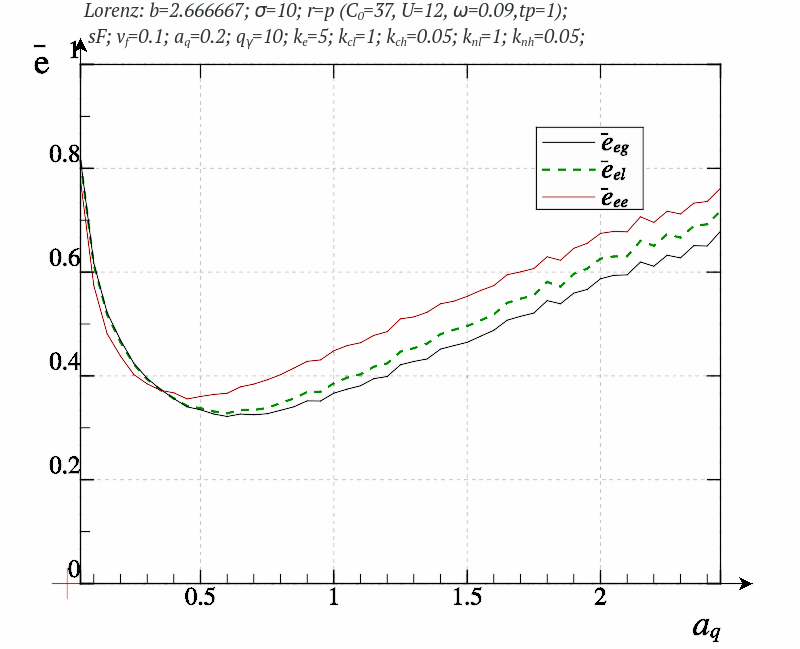
\includegraphics[width=0.49\textwidth]{p/cha/lor/Fq3zlovnAAF/lor_Fq3zlovnAAF_qx2-p_a_q_e_sign.png}
    \hfill
    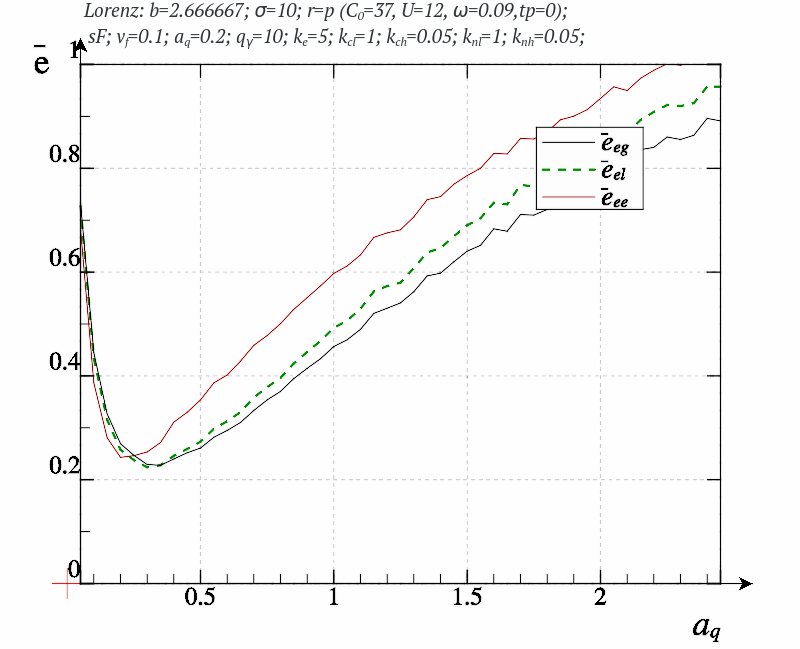
\includegraphics[width=0.49\textwidth]{p/cha/lor/Fq3zlovnAAF/lor_Fq3zlovnAAF_qx2-p_a_q_e_sin.png}
  }
  \caption{Зависимости $\overline{e}_{r*}(a_q)$ при идентификации системы Лоренца методом Fq3zlovnAAF.$q_{x^2}$
   при~(\ref{atu:eq:lor_po_t_sign}) и (\ref{atu:eq:lor_po_t_sin})}
  \label{atu:f:lor_a_q_Fq3zlovnAAF.q_x2}
\end{figure}


Следующий важные параметр -- масштаб функции качества $q_\gamma$.
В первую очередь он должен влиять на методы,
которые используют величину $F$ в процессе поиска.
С другой стороны, методы, использующие только критерий для
определения $p_e$, тоже используют  $q_\gamma$ в процессе
определения $p_{id}$.

На рис.~\ref{atu:f:lor_qg_ql3ruonAAF.q_x2} представлены зависимости
усреднённых ошибок идентификации системы Лоренца от $q_\gamma$ при использовании метода ql3ruonAAF.$q_{x^2}$.
Как и предполагалось, зависимости достаточно слабые, за исключением $\overline{e}_{rge}$,
для которой большие величины масштаба обозначают малую чувствительность,
и следовательно, избыточное влияние агентов, расположенных
вдали от искомого значения параметра.
Самые устойчиво хорошие результаты демонстрирует $p_{ee}$.

\begin{figure}[ht!]
  \centerline{
    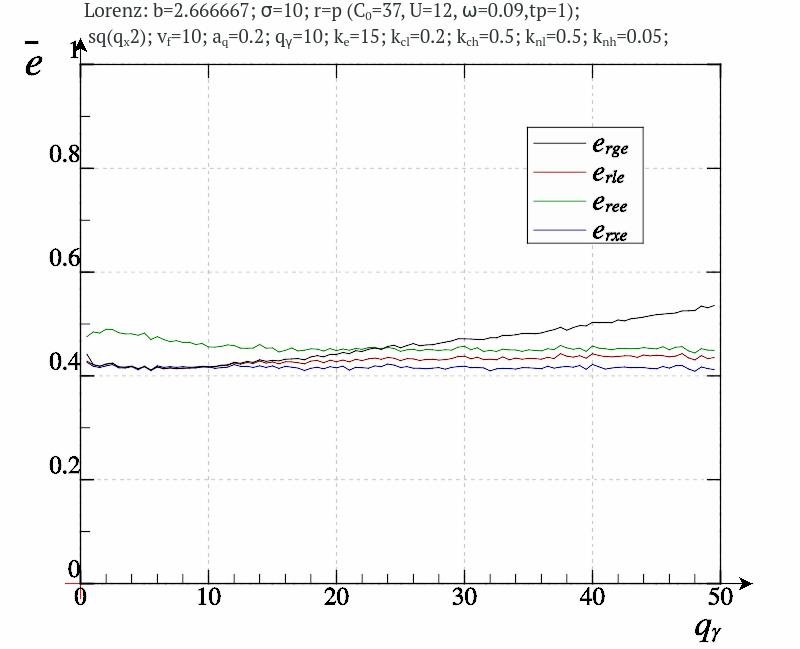
\includegraphics[width=0.49\textwidth]{p/cha/lor/ql3ruonAAF/lor_ql3ruonAAF_qx2-p_qgamma_e_sign.png}
    \hfill
    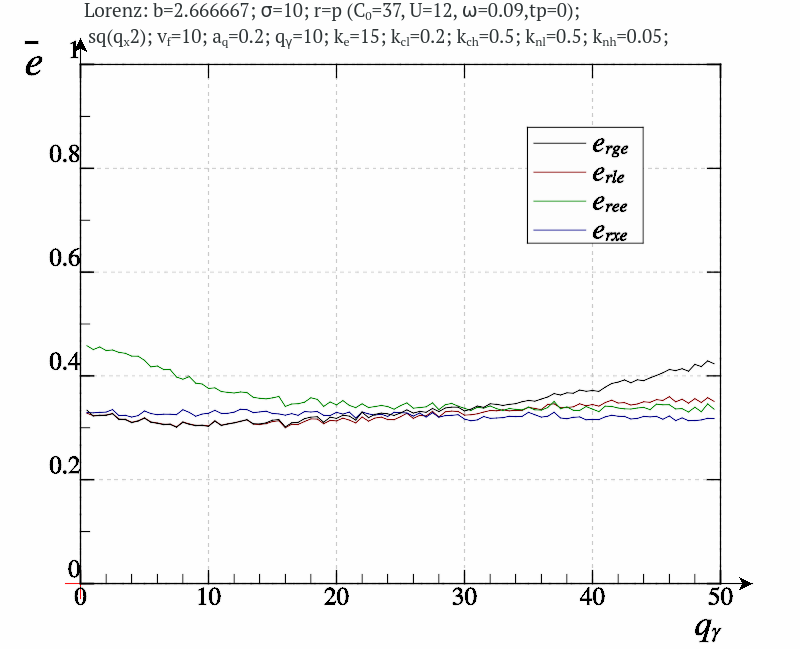
\includegraphics[width=0.49\textwidth]{p/cha/lor/ql3ruonAAF/lor_ql3ruonAAF_qx2-p_qgamma_e_sin.png}
  }
  \caption{Зависимости $\overline{e}_{r*}(q_\gamma)$ при идентификации системы Лоренца методом ql3ruonAAF.$q_{x^2}$
   при~(\ref{atu:eq:lor_po_t_sign}) и (\ref{atu:eq:lor_po_t_sin})}
  \label{atu:f:lor_qg_ql3ruonAAF.q_x2}
\end{figure}



На рис.~\ref{atu:f:lor_qg_ql3ruonAAF.q_y2} представлены зависимости
усреднённых ошибок идентификации системы Лоренца от $q_\gamma$ при использовании метода ql3ruonAAF.$q_{y^2}$.
Здесь результаты аналогичны предыдущему случаю. Однако,
данный подход оказался более чувствительным к заниженным значением $q_\gamma$.

\begin{figure}[ht!]
  \centerline{
    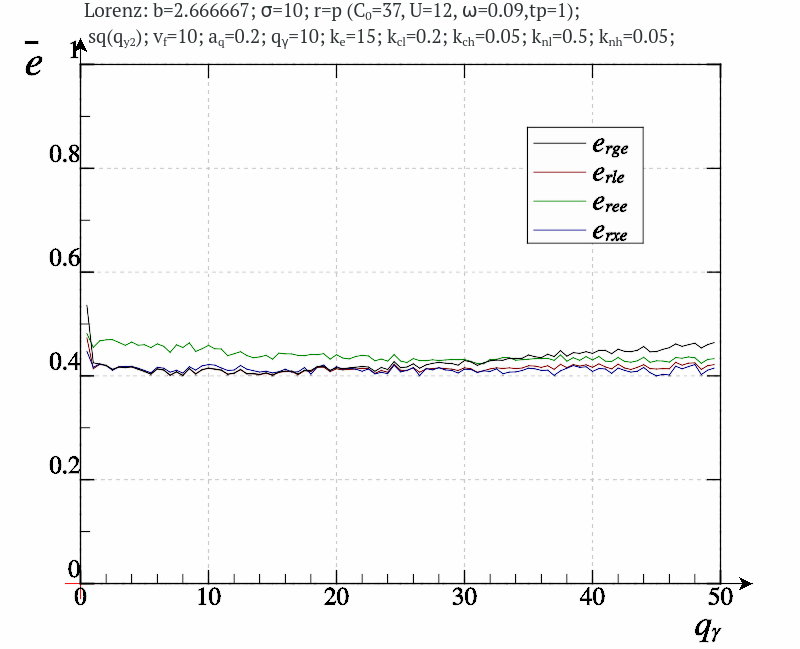
\includegraphics[width=0.49\textwidth]{p/cha/lor/ql3ruonAAF/lor_ql3ruonAAF_qy2-p_qgamma_e_sign.png}
    \hfill
    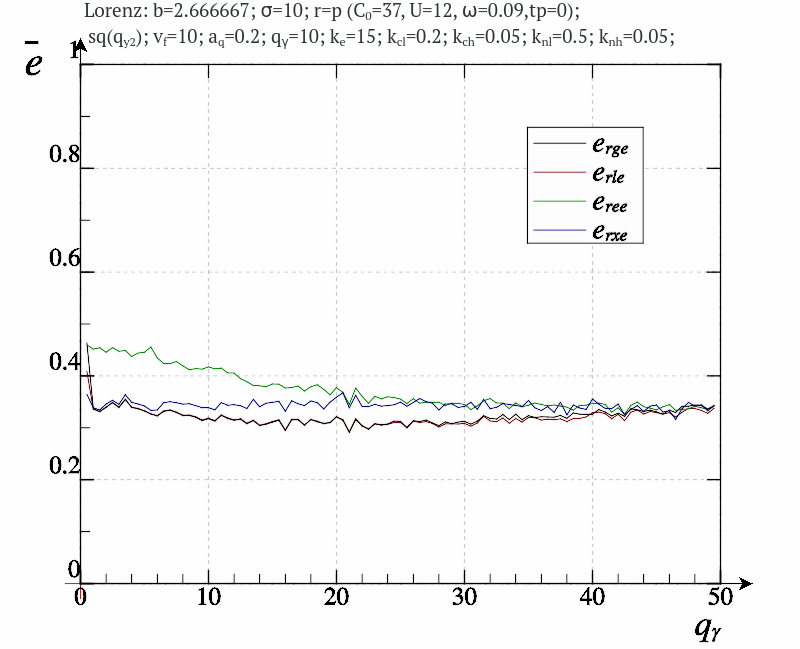
\includegraphics[width=0.49\textwidth]{p/cha/lor/ql3ruonAAF/lor_ql3ruonAAF_qy2-p_qgamma_e_sin.png}
  }
  \caption{Зависимости $\overline{e}_{r*}(q_\gamma)$ при идентификации системы Лоренца методом ql3ruonAAF.$q_{y^2}$
   при~(\ref{atu:eq:lor_po_t_sign}) и (\ref{atu:eq:lor_po_t_sin})}
  \label{atu:f:lor_qg_ql3ruonAAF.q_y2}
\end{figure}


На рис.~\ref{atu:f:lor_qg_Fq3zlovnAAF.q_x2} представлены зависимости
усреднённых ошибок идентификации системы Лоренца от $q_\gamma$ при использовании метода FAlv.3z.$q_{x^2}$.
В этом случае зависимости сильно отличаются от двух предыдущих случаев.
Так как этот метод непосредственно используют функцию
качества для определения $p_e$ каждым агентом, то зависимость
имеет явный экстремальный характер.
При малых значениях $q_\gamma$ чувствительность избыточна,
и процесс поиска нарушается.
При больших -- недостаточна, и помимо избыточного влияния ``дальних'' агентов также снижается скорость и точность поиска.
Влияние  ``дальних'' агентов игнорируется при использовании
$p_{le}$ и $p_{ee}$, однако,
в эти методы теряются точность при переключении
между лучшими агентами.


\begin{figure}[ht!]
  \centerline{
    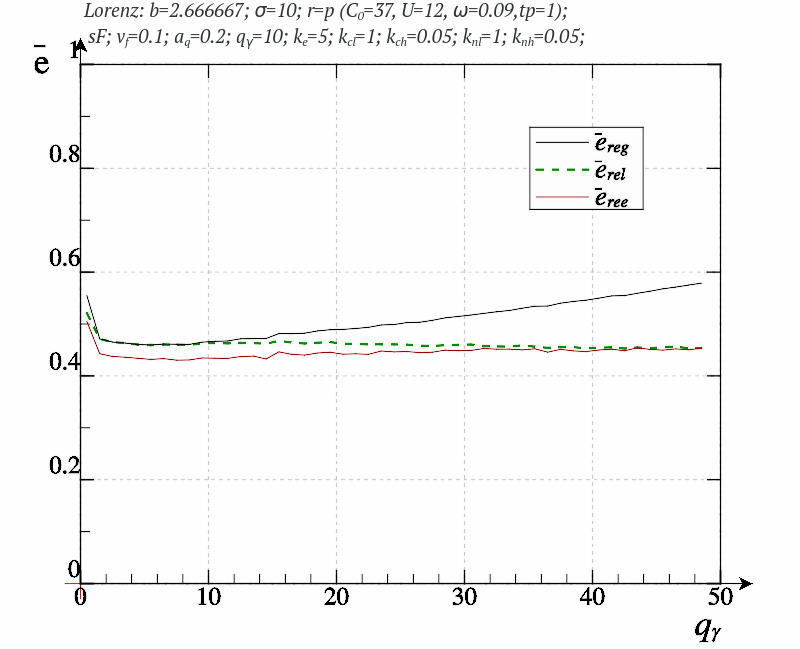
\includegraphics[width=0.49\textwidth]{p/cha/lor/Fq3zlovnAAF/lor_Fq3zlovnAAF_qx2-p_qg_e_sign.png}
    \hfill
    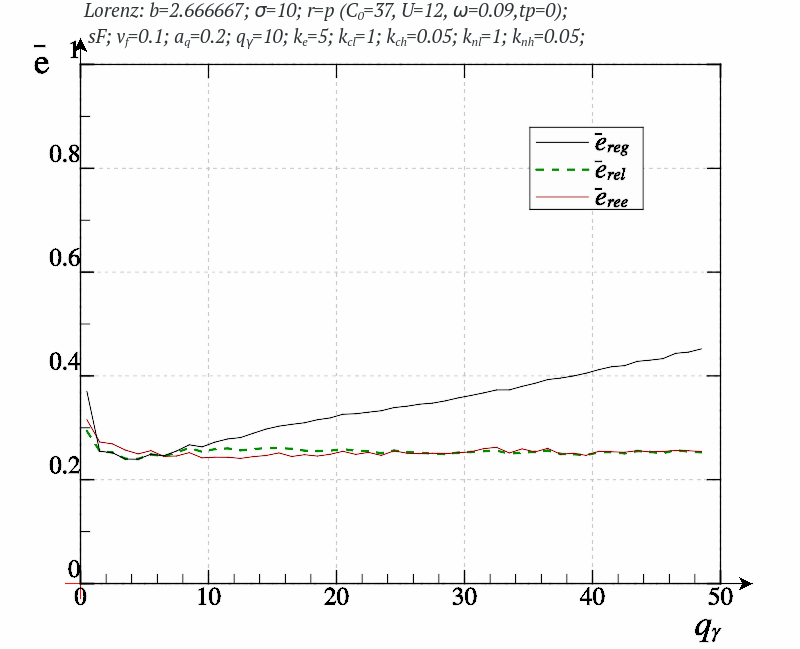
\includegraphics[width=0.49\textwidth]{p/cha/lor/Fq3zlovnAAF/lor_Fq3zlovnAAF_qx2-p_qg_e_sin.png}
  }
  \caption{Зависимости $\overline{e}_{r*}(q_\gamma)$ при идентификации системы Лоренца методом Fq3zlovnAAF.$q_{x^2}$
   при~(\ref{atu:eq:lor_po_t_sign}) и (\ref{atu:eq:lor_po_t_sin})}
  \label{atu:f:lor_qg_Fq3zlovnAAF.q_x2}
\end{figure}


Ещё один важный параметр, влияющий на динамический свойства
системы идентификации -- $v_f$, определяющий скорость
смещения агента к выбранному значению при постоянной силе.
При нулевом значении этого коэффициента агенты неподвижны,
и можно определить величину $\overline{e}_{be}$,
а если ещё предельно уменьшить $q_\gamma$ --  $\overline{e}_{bb}$.



На рис.~\ref{atu:f:lor_vf_ql3ruonAAF.q_x2} представлены зависимости
усреднённых ошибок идентификации системы Лоренца от $v_f$ при использовании метода ql3ruonAAF.$q_{x^2}$.
За исключением начального участка, где подвижность агентов
минимальна, зависимость от $v_f$ достаточно слабая.
По мере увеличения $v_f$ немного улучшаются динамические свойства,
но возрастающая скорость перемещения агентов
несколько нивелирует этот эффект. При плавном изменении параметра,
негативный эффект от избыточной подвижности агентов преобладает.

\begin{figure}[ht!]
  \centerline{
    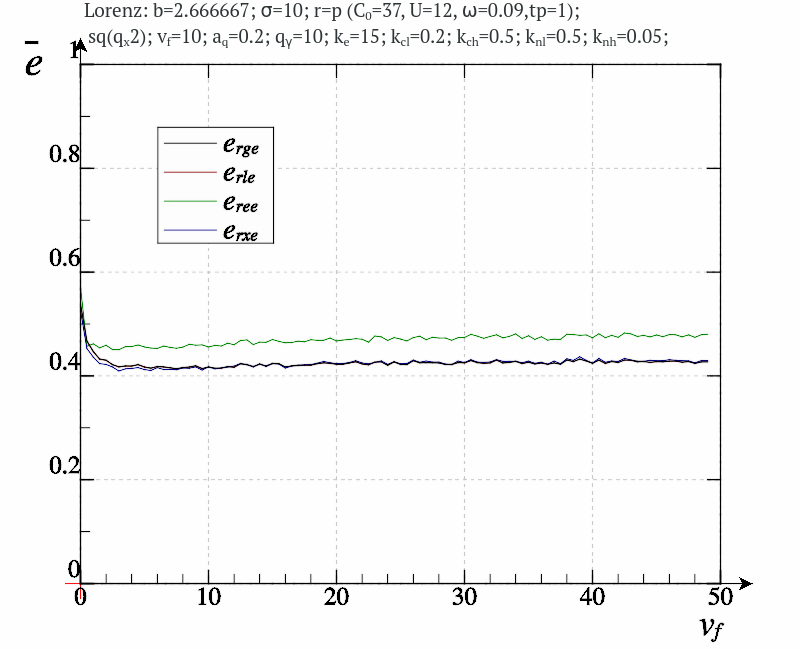
\includegraphics[width=0.49\textwidth]{p/cha/lor/ql3ruonAAF/lor_ql3ruonAAF_qx2-p_v_f_e_sign.png}
    \hfill
    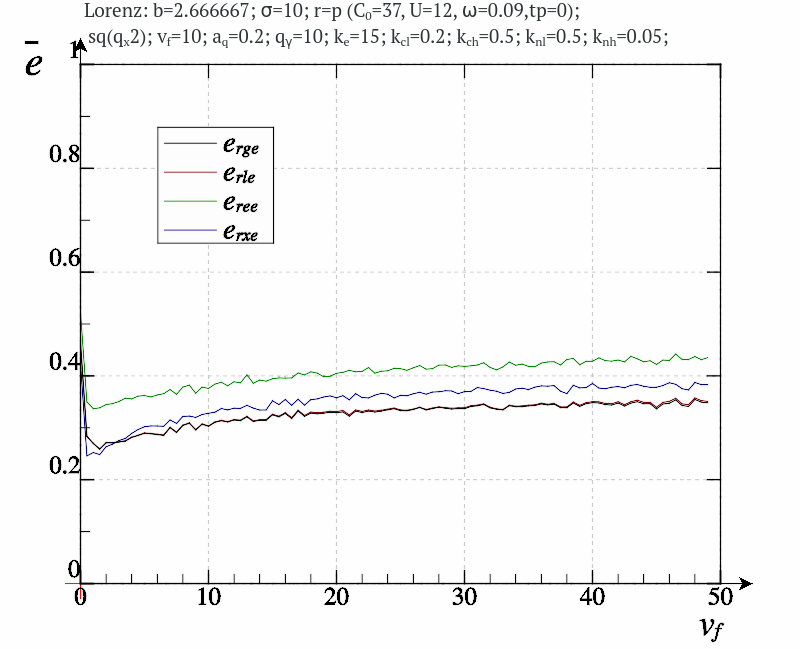
\includegraphics[width=0.49\textwidth]{p/cha/lor/ql3ruonAAF/lor_ql3ruonAAF_qx2-p_v_f_e_sin.png}
  }
  \caption{Зависимости $\overline{e}_{r*}(v_f)$ при идентификации системы Лоренца методом ql3ruonAAF.$q_{x^2}$
   при~(\ref{atu:eq:lor_po_t_sign}) и (\ref{atu:eq:lor_po_t_sin})}
  \label{atu:f:lor_vf_ql3ruonAAF.q_x2}
\end{figure}

Совершенно аналогичная картина
(рис.~\ref{atu:f:lor_vf_ql3ruonAAF.q_y2})
наблюдается при использовании критерия $q_{y^2}$.
При этом следует отметить, что при избыточной подвижности
меньшее значение ошибки демонстрируют
подход, основанные на глобальном оценивании $p_{id}$.


\begin{figure}[ht!]
  \centerline{
    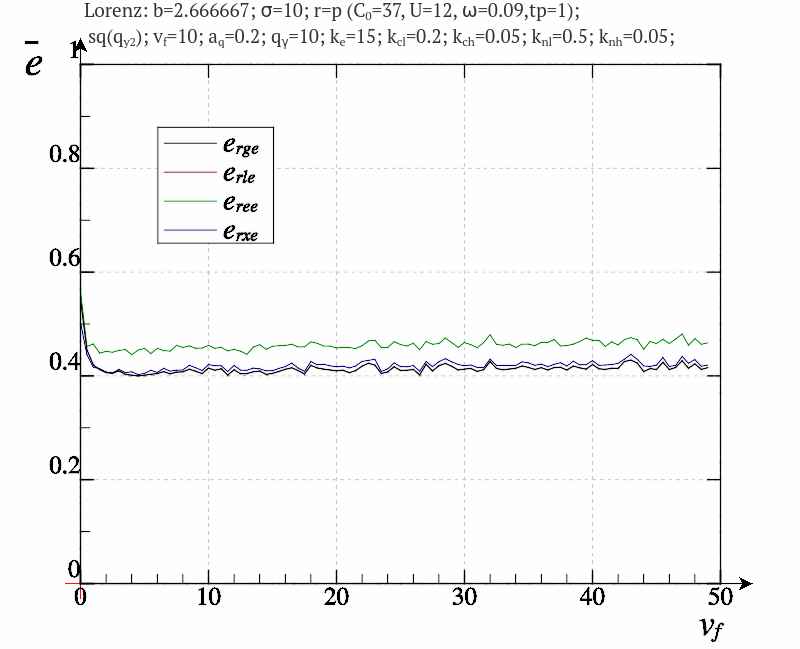
\includegraphics[width=0.49\textwidth]{p/cha/lor/ql3ruonAAF/lor_ql3ruonAAF_qy2-p_v_f_e_sign.png}
    \hfill
    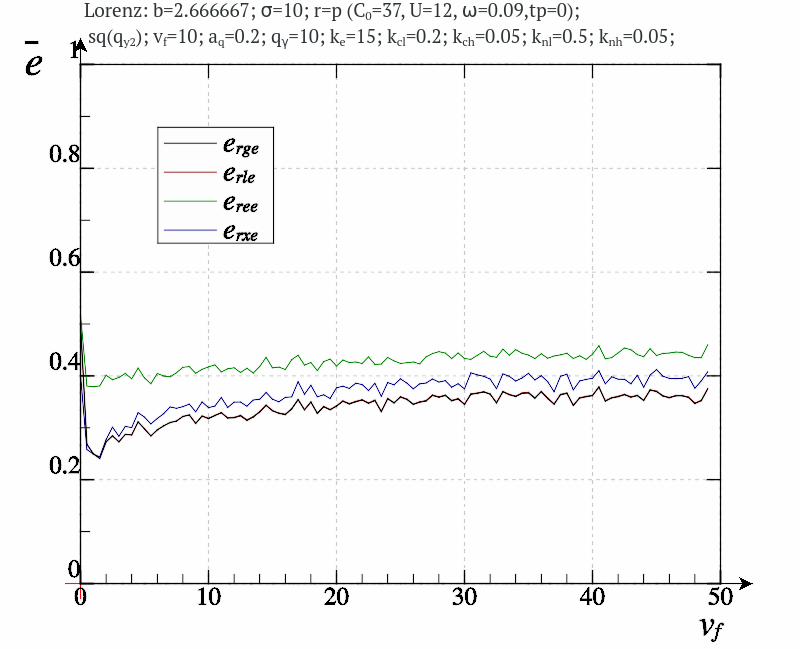
\includegraphics[width=0.49\textwidth]{p/cha/lor/ql3ruonAAF/lor_ql3ruonAAF_qy2-p_v_f_e_sin.png}
  }
  \caption{Зависимости $\overline{e}_{r*}(v_f)$ при идентификации системы Лоренца методом ql3ruonAAF.$q_{y^2}$
   при~(\ref{atu:eq:lor_po_t_sign}) и (\ref{atu:eq:lor_po_t_sin})}
  \label{atu:f:lor_vf_ql3ruonAAF.q_y2}
\end{figure}

Несколько другая картина наблюдается при использовании метода  Fq3zlovnAAF.$q_{x^2}$
(рис.~\ref{atu:f:lor_vf_Fq3zlovnAAF.q_x2}).
В достаточно широком диапазоне зависимость достаточно слабая,
а большая скорость приводит к нарушению процесса поиска,
что наблюдается в правой части обеих графиков.

\begin{figure}[ht!]
  \centerline{
    \includegraphics[width=0.49\textwidth]{p/cha/lor/Fq3zlovnAAF/lor_Fq3zlovnAAF_qx2-p_v_f_e_sign.png}
    \hfill
    \includegraphics[width=0.49\textwidth]{p/cha/lor/Fq3zlovnAAF/lor_Fq3zlovnAAF_qx2-p_v_f_e_sin.png}
  }
  \caption{Зависимости $\overline{e}_{r*}(v_f)$ при идентификации системы Лоренца методом Fq3zlovnAAF.$q_{x^2}$
   при~(\ref{atu:eq:lor_po_t_sign}) и (\ref{atu:eq:lor_po_t_sin})}
  \label{atu:f:lor_vf_Fq3zlovnAAF.q_x2}
\end{figure}

Последний из заслуживающих пристального внимания параметр -- $k_e$,
определяющий баланс сил при смещении агентов.
Следует отметить, что в рассматриваемых примерах его влияние различное --
в ql3ruonAAF.$q_{x^2}$ и ql3ruonAAF.$q_{y^2}$
зависимость $f_e(p_c-p_e)$ с насыщением,
а в Fq3zlovnAAF.$q_{x^2}$ эта зависимость линейная.

На рис.~\ref{atu:f:lor_ke_ql3ruonAAF.q_x2} представлены зависимости
усреднённых ошибок идентификации системы Лоренца от $k_e$ при использовании метода ql3ruonAAF.$q_{x^2}$.
Малые значения этого коэффициента приводят к там же последствиям, что и малые
значения $v_f$ -- агенты становятся практически неподвижными.

\begin{figure}[ht!]
  \centerline{
    \includegraphics[width=0.49\textwidth]{p/cha/lor/ql3ruonAAF/lor_ql3ruonAAF_qx2-p_k_e_e_sign.png}
    \hfill
    \includegraphics[width=0.49\textwidth]{p/cha/lor/ql3ruonAAF/lor_ql3ruonAAF_qx2-p_k_e_e_sin.png}
  }
  \caption{Зависимости $\overline{e}_{r*}(k_e)$ при идентификации системы Лоренца методом ql3ruonAAF.$q_{x^2}$
   при~(\ref{atu:eq:lor_po_t_sign}) и (\ref{atu:eq:lor_po_t_sin})}
  \label{atu:f:lor_ke_ql3ruonAAF.q_x2}
\end{figure}

Нарушение процесса поиска при использовании критерия $q_{y^2}$~рис.~\ref{atu:f:lor_ke_ql3ruonAAF.q_y2}
происходит заметно раньше, чем при использовании $q_y^2$. Это
ещё раз подтверждает меньший диапазон пригодности $q_{y^2}$.

\begin{figure}[ht!]
  \centerline{
    \includegraphics[width=0.49\textwidth]{p/cha/lor/ql3ruonAAF/lor_ql3ruonAAF_qy2-p_k_e_e_sign.png}
    \hfill
    \includegraphics[width=0.49\textwidth]{p/cha/lor/ql3ruonAAF/lor_ql3ruonAAF_qy2-p_k_e_e_sin.png}
  }
  \caption{Зависимости $\overline{e}_{r*}(k_e)$ при идентификации системы Лоренца методом ql3ruonAAF.$q_{y^2}$
   при~(\ref{atu:eq:lor_po_t_sign}) и (\ref{atu:eq:lor_po_t_sin})}
  \label{atu:f:lor_ke_ql3ruonAAF.q_y2}
\end{figure}

На рис.~\ref{atu:f:lor_ke_Fq3zlovnAAF.q_x2} представлены аналогичные зависимости
для метода  Fq3zlovnAAF.$q_{x^2}$. При общей подобной структуре зависимости
не наблюдается нарушение поиска и при вдвое большем значении данного коэффициента.

\begin{figure}[ht!]
  \centerline{
    \includegraphics[width=0.49\textwidth]{p/cha/lor/Fq3zlovnAAF/lor_Fq3zlovnAAF_qx2-p_ke_e_sign.png}
    \hfill
    \includegraphics[width=0.49\textwidth]{p/cha/lor/Fq3zlovnAAF/lor_Fq3zlovnAAF_qx2-p_ke_e_sin.png}
  }
  \caption{Зависимости $\overline{e}_{r*}(k_e)$ при идентификации системы Лоренца методом Fq3zlovnAAF.$q_{x^2}$
   при~(\ref{atu:eq:lor_po_t_sign}) и (\ref{atu:eq:lor_po_t_sin})}
  \label{atu:f:lor_ke_Fq3zlovnAAF.q_x2}
\end{figure}

% }}}2


% ----------------------------------------- F_type -------------------------------

\subsection{Влияние вида функции качества на процесс идентификации}  % {{{2

Рассмотрим влияние типа функции качества на свойства системы идентификации.
Для этого рассмотрим семейство зависимостей
$\overline{e}(q_\gamma)$ для различных видов $F(q)$
(\ref{atu:eq:F_gauss})--(\ref{atu:eq:F_log}).
Для данного исследования выбран метод Fq3zlovnAAF.$q_{x^2}$,
как напрямую использующий функцию качества при
аппроксимации $p_e$.
Из всех видов зависимостей выбранны именно эти,
так как $q_\gamma$ непосредственно входит в определение функции качества.


На рис.~\ref{atu:f:lor_ftype_rge} представлены $\overline{e}_{rge}(q_\gamma)$ 
при использовании метода  Fq3zlovnAAF.$q_{x^2}$.
Следует отметить, что в этом случае функция качества используется два раза:
первый раз в каждом агенте при определении $p_e$,
второй -- при определении глобального $p_{ge}$.
Именно это влияние объясняет плавный прост ошибки идентификации
при росте $q_\gamma$, и следовательно, уменьшению чувствительности в правой части графиков.
В левой части графиков наблюдаются существенные различия
при использовании различных видов функций качества.
Применение параболической, треугольной и логарифмической зависимостей
приводит к резкому росту ошибки при увеличении чувствительности.
Гиперболическая и Гауссовая зависимости остаются применимы и при
завышенной чувствительности функции качества.

\begin{figure}[ht!]
  \centerline{
    \includegraphics[width=0.49\textwidth]{p/cha/lor/Fq3zlovnAAF/f_type/lor_Fq3zlovnAAF_qx2_Ft-p_qg_e_all_sign_rge.png}
    \hfill
    \includegraphics[width=0.49\textwidth]{p/cha/lor/Fq3zlovnAAF/f_type/lor_Fq3zlovnAAF_qx2_Ft-p_qg_e_all_sin_rge.png}
  }
  \caption{Семейства зависимостей $\overline{e}_{rge}(q_\gamma)$ для различных видов функций качества при идентификации системы Лоренца методом Fq3zlovnAAF.$q_{x^2}$
   при~(\ref{atu:eq:lor_po_t_sign}) и (\ref{atu:eq:lor_po_t_sin})}
  \label{atu:f:lor_ftype_rge}
\end{figure}

На рис.~\ref{atu:f:lor_ftype_ree} представлены $\overline{e}_{rge}(q_\gamma)$
при использовании метода  Fq3zlovnAAF.$q_{x^2}$.
Результаты в целом схожи с предыдущими, список видов функций качества, обеспечивающих
более широкий диапазон применимости не изменился. Тем не менее, ввиду того,
что в данном случае используется только локальная оценка, рост
$q_\gamma$ в разумных пределах не приводит к увеличению ошибки идентификации.

\begin{figure}[ht!]
  \centerline{
    \includegraphics[width=0.49\textwidth]{p/cha/lor/Fq3zlovnAAF/f_type/lor_Fq3zlovnAAF_qx2_Ft-p_qg_e_all_sign_ree.png}
    \hfill
    \includegraphics[width=0.49\textwidth]{p/cha/lor/Fq3zlovnAAF/f_type/lor_Fq3zlovnAAF_qx2_Ft-p_qg_e_all_sin_ree.png}
  }
  \caption{Семейства зависимостей $\overline{e}_{ree}(q_\gamma)$ для различных видов функций качества при идентификации системы Лоренца методом Fq3zlovnAAF.$q_{x^2}$
   при~(\ref{atu:eq:lor_po_t_sign}) и (\ref{atu:eq:lor_po_t_sin})}
  \label{atu:f:lor_ftype_ree}
\end{figure}

Таким образом, результаты моделирования при использовании
функций качества видов
(\ref{atu:eq:F_gauss})--(\ref{atu:eq:F_log}) показывают,
что при сравнительно одинаковых результатах в широком
диапазоне $q_\gamma$, лучшие результаты в целом
демонстрируют функции (\ref{atu:eq:F_hyper}) и (\ref{atu:eq:F_gauss}),
за счёт лучшей работы в области высокой чувствительности.
А так как в целом применение гиперболической зависимости
приводит пусть к несущественно, но большей ошибке идентификации в целом,
то в дальнейшем будем применять функцию качества в виде~(\ref{atu:eq:F_gauss}).

% }}}2


% ----------------------------------------- N -------------------------------

\subsection{Влияние количества поисковых агентов на процесс идентификации}  % {{{2

Рассмотрим влияние количества поисковых агентов
на качество идентификации на примере семейства методов Fq3zlovnAAF.$q_{x^2}$.
Структура связей поисковых агентов определяет их минимальное количество $N=3$,
не считая двух неподвижных моделей на границах.
Рассмотрим случаи $N=3,5,7,9$.

В первую очередь отметим,
что из всех параметров рассматриваемой системы идентификации
наиболее тесную и непосредственную связь с количеством
агентов имеет параметр $q_\gamma$. Что должно объясняется тем, что чем больше
агентов на $\mathcal{P}$, тем меньше между ними расстояние в пространстве параметров,
и следовательно, значения критериев идентификации различаются меньше,
что, в свою очередь, требует большей чувствительности.

Рассмотрим получившиеся зависимости.
На рис.~\ref{atu:f:lor_N_rge} представлены $\overline{e}_{rge}(q_\gamma)$
для различных $N$. Здесь получены, на первый взгляд, парадоксальные результаты.
В обеих случаях, при относительно больших значениях $q_\gamma$,
система идентификации с тремя моделями показывает лучшие результаты.
На самом деле, никакого парадокса в полученных данных нет.
При определении $p_{ge}$, а следовательно, а $\overline{e}_{rge}$
учитывается вклад всех моделей, в том числе и расположенных далеко от $p_o$.
При больших значениях $q_\gamma$, и следовательно, при низкой чувствительности,
вклад ``дальних'' моделей возрастает, и, чем больше моделей,
тем больше этот вклад. При нормальной чувствительности (левая часть графиков),
этот эффект практически пропадает. Тем не менее, для данных условий,
использование количества моделей $N>5$ нецелесообразно.



\begin{figure}[ht!]
  \centerline{
    \includegraphics[width=0.49\textwidth]{p/cha/lor/Fq3zlovnAAF/N/lor_Fq3zlovnAAF_qx2_p_qg_e_rge_sign.png}
    \hfill
    \includegraphics[width=0.49\textwidth]{p/cha/lor/Fq3zlovnAAF/N/lor_Fq3zlovnAAF_qx2_p_qg_e_rge_sin.png}
  }
  \caption{Семейства зависимостей $\overline{e}_{rge}(q_\gamma)$ для различных значений $N$ при идентификации системы Лоренца методом Fq3zlovnAAF.$q_{x^2}$
   при~(\ref{atu:eq:lor_po_t_sign}) и (\ref{atu:eq:lor_po_t_sin})}
  \label{atu:f:lor_N_rge}
\end{figure}


Применение локальных методов оценивания $p_\mathrm{id}$,
с ограниченным количеством используемых моделей, не должно быть подвержено
этому явлению. Для проверки этого тезиса рассмотрим зависимости
$\overline{e}_{ree}(q_\gamma)$
представленные на рис.~\ref{atu:f:lor_N_rge}
для того же набора $N$.

\begin{figure}[ht!]
  \centerline{
    \includegraphics[width=0.49\textwidth]{p/cha/lor/Fq3zlovnAAF/N/lor_Fq3zlovnAAF_qx2_p_qg_e_ree_sign.png}
    \hfill
    \includegraphics[width=0.49\textwidth]{p/cha/lor/Fq3zlovnAAF/N/lor_Fq3zlovnAAF_qx2_p_qg_e_ree_sin.png}
  }
  \caption{Семейства зависимостей $\overline{e}_{ree}(q_\gamma)$ для различных значений $N$ при идентификации системы Лоренца методом Fq3zlovnAAF.$q_{x^2}$
   при~(\ref{atu:eq:lor_po_t_sign}) и (\ref{atu:eq:lor_po_t_sin})}
  \label{atu:f:lor_N_ree}
\end{figure}

В этом случае при больших значениях $q_\gamma$ все рассматриваемые ошибки идентификации
практически совпадают, и проявляют достаточно слабую зависимость.
В левой части графиков, система с $N=3$ заметно
проигрывает системе с $N=5$, а остальные не превосходят последнюю.

\Cmt{TODO: Обосновать такое ограничение}



% }}}2


% ----------------------------------------- multi param -------------------------------

\subsection{Зависимости значений критериев идентификации при изменении двух параметров системы Лоренца}  % {{{2

Для оценивания возможности одновременной идентификации нескольких параметров
рассмотрим графики зависимостей критериев, но при условии
изменения двух параметров попарно: ($r$,$\sigma$) и ($r$,$b$).
При этом воспользуется структурой системы ~(\ref{atu:eq:lor})
и введём ещё один дополнительный критерий: $q_{(x-y)^2}$.

На рис.~\ref{atu:f:lor_qx2_r_b} приведена зависимость
$q_{x^2}(r,b)$.
Анализ вида этой поверхности позволяет сделать вывод,
что одного этого критерия недостаточно для
одновременной идентификации параметров $r$ и $b$.
Явно выраженный ``овраг'' на графике соответствует
переходу из режима затухания в хаотический,
следовательно, не имеет принципиального значения.

\begin{figure}[ht!]
  \centerline{  \includegraphics[width=0.60\textwidth]{p/cha/lor/q2d/lor_qx2_r_b.png}  }
  \caption{Зависимость $q_{x^2}(r,b)$ для системы Лоренца}
  \label{atu:f:lor_qx2_r_b}
\end{figure}


На рис.~\ref{atu:f:lor_qy2_r_b} приведена зависимость
$q_{y^2}(r,b)$. Вид этой поверхности практически не отличается от предыдущей.
При этом совершенно не наблюдается никаких очевидных причин обнаруженному
в предыдущих исследованиях
более узкому диапазону применимости данного критерия.

\begin{figure}[ht!]
  \centerline{  \includegraphics[width=0.60\textwidth]{p/cha/lor/q2d/lor_qy2_r_b.png}  }
  \caption{Зависимость $q_{y^2}(r,b)$ для системы Лоренца}
  \label{atu:f:lor_qy2_r_b}
\end{figure}

На рис.~\ref{atu:f:lor_qz2_r_b} приведена зависимость
$q_{z^2}(r,b)$.
Вид данная зависимости существенно отличается от двух предыдущих.
Близкая к квадратичной зависимость от параметра $r$
не представляет особых проблем. Полезным является тот факт,
что для данного критерия зависимость от параметра $b$
достаточно мала. Следовательно, при двупараметрической идентификации
данный критерий имеет смысл  использовать для (оценочной)
идентификации параметра $r$, и совокупность данного критерия
вместе с, например, $q_{x^2}$ позволит идентифицировать
оба параметра без избыточного количества моделей.

\begin{figure}[ht!]
  \centerline{  \includegraphics[width=0.60\textwidth]{p/cha/lor/q2d/lor_qz2_r_b.png}  }
  \caption{Зависимость $q_{z^2}(r,b)$ для системы Лоренца}
  \label{atu:f:lor_qz2_r_b}
\end{figure}

На рис.~\ref{atu:f:lor_qxmy2_r_b} приведена зависимость
$q_{(x-y)^2}(r,b)$.
Очевидно, что для идентификации данный критерий
практически непригоден, тем не менее,
он отличен от нуля только там, где системы не
находится в режиме затухания, что может быть полезно
для быстрого определения режима работы.

\begin{figure}[ht!]
  \centerline{  \includegraphics[width=0.60\textwidth]{p/cha/lor/q2d/lor_qxmy2_r_b.png}  }
  \caption{Зависимость $q_{(x-y)^2}(r,b)$ для системы Лоренца}
  \label{atu:f:lor_qxmy2_r_b}
\end{figure}


На рис.~\ref{atu:f:lor_qx2_r_sigma} приведена зависимость
$q_{x^2}(r,\sigma)$.
Поведение этого критерия на паре параметров $(r,\sigma)$
существенно отличается от его же поведения на паре $(r,b)$.
За исключением узкого ``оврага'', зависимость от параметра $\sigma$
пренебрежимо мала, что даёт основания для
независимой идентификации параметра~$r$.

\begin{figure}[ht!]
  \centerline{  \includegraphics[width=0.60\textwidth]{p/cha/lor/q2d/lor_qx2_r_sigma.png}  }
  \caption{Зависимость $q_{x^2}(r,\sigma)$ для системы Лоренца}
  \label{atu:f:lor_qx2_r_sigma}
\end{figure}


На рис.~\ref{atu:f:lor_qy2_r_sigma} приведена зависимость
$q_{y^2}(r,\sigma)$.
Эта зависимость в целом похожа на предыдущую,
однако, на месте ``оврага'' наблюдается ``хребет''.

\begin{figure}[ht!]
  \centerline{  \includegraphics[width=0.60\textwidth]{p/cha/lor/q2d/lor_qy2_r_sigma.png}  }
  \caption{Зависимость $q_{y^2}(r,\sigma)$ для системы Лоренца}
  \label{atu:f:lor_qy2_r_sigma}
\end{figure}

На рис.~\ref{atu:f:lor_qz2_r_sigma} приведена зависимость
$q_{z^2}(r,\sigma)$. В отличие от применения данного
критерия на паре $(r,b)$, не наблюдается принципиальной
разницы между данным критерием, и критерием $q_{x^2}$.
Отсутствие существенного различия не даёт достаточных
оснований для одновременной идентификации
пары параметров $(r,\sigma)$ с применением только этих
двух критериев.

\begin{figure}[ht!]
  \centerline{  \includegraphics[width=0.60\textwidth]{p/cha/lor/q2d/lor_qz2_r_sigma.png}  }
  \caption{Зависимость $q_{z^2}(r,\sigma)$ для системы Лоренца}
  \label{atu:f:lor_qz2_r_sigma}
\end{figure}

На рис.~\ref{atu:f:lor_qxmy2_r_sigma} приведена зависимость
$q_{(x-y)^2}(r,\sigma)$. Эта зависимость принципиально не отличается
от представленной на рис.~(\ref{atu:f:lor_qxmy2_r_b}),
за исключением того, что присутствует ``хребет''.

\begin{figure}[ht!]
  \centerline{  \includegraphics[width=0.60\textwidth]{p/cha/lor/q2d/lor_qxmy2_r_sigma.png}  }
  \caption{Зависимость $q_{(x-y)^2}(r,\sigma)$ для системы Лоренца}
  \label{atu:f:lor_qxmy2_r_sigma}
\end{figure}

% }}}2


\subsection{Выводы}  % {{{2

Результаты моделирования как собственно динамики
системы Лоренца,
так и процессов идентификации параметра ``$r$''
позволяют в целом сделать следующие выводы:

\begin{itemize}

  \item
    Для синтеза работоспособной системы идентификации параметра  ``$r$''
    системы Лоренца могут применяться практически всё рассмотренные критерии.
    При этом, больший диапазон применимости -- у критерия~$q_{x^2}$.

  \item
    Система мультиагентной идентификации может быть
    реализована как с агентами, осуществляющими поиск
    как с использованием критерия, так и с использованием
    функции качества. При этом, ошибка идентификации
    определяется в основном не конкретным методом,
    а динамическими свойствами самого идентифицируемого
    объекта и используемым временем усреднения критерия.

  \item
    Для рассматриваемого типа объектов большинство параметров
    системы идентификации допускают изменение в достаточно
    широком диапазоне без потери работоспособности,
    что упрощает применение системы идентификации
    в случаях, когда нет возможности проводить
    широкий набор предварительных измерений.
    Исключением является параметр $a_q$, при этом его допустимый диапазон
    определяется динамическим свойствами объекта.

  \item
    Применение функции качества в виде~(\ref{atu:eq:F_gauss})
    позволяет в целом получить лучшие результаты идентификации.

  \item
    Существует определённое количество агентов,
    превышение которого не увеличивает качество идентификации,
    а в некоторых случаях, например, при использовании глобальных
    методов оценивания $p_{id}$ и низкой чувствительности,
    приводит к ухудшению свойств системы идентификации.

  \item
    Возможна одновременная идентификация параметров $r$ и $b$,
    при условии совместного применения критериев $q_{x^2}$ и $q_{z^2}$.

\end{itemize}

% }}}2


% }}}1




% habr: 
% 1. Конвекция в тороидальной трубе (Ланда П.С. Нелинейные колебания и волны. — М: Либроком, 2010, с. 454-455)
% 2. Одномодовый лазер (Покровский Л.А. Решение системы уравнений Лоренца в
%  асимптотическом пределе большого числа Релея. I. Система Лоренца в простейшей
%  квантовой модели лазера и приложение к ней метода усреднения // Теоретическая
%  и математическая физика, 1985, т. 62, №2, с. 272-290);
% 3. Осциллятор с инерционным возбуждением (Неймарк Ю.И., Ланда П.С.
% Стохастические и хаотические колебания. — М: Либроком, 2009, с. 288-295).

% vim: fdm=marker foldlevel=1 foldignore="%#" fdc=4 ft=tex
